\documentclass[aspectratio=169]{beamer}

% ── Packages ──────────────────────────────────────────────────────────────────
\usepackage{tikz}
\usetikzlibrary{positioning,arrows.meta,fit,backgrounds}
\usepackage{graphicx}
\usepackage{booktabs}
\usepackage{xcolor}
\usepackage{fontenc}
\usepackage{lmodern}
\usepackage{microtype}
\usepackage{amsmath,amssymb}
\usepackage{adjustbox}
\usepackage{pgfplots}
\pgfplotsset{compat=1.18}

% ── Color Palette (from CRR-Pipeline-Build-Flowchart) ─────────────────────────
\definecolor{navydark}{RGB}{10,22,40}
\definecolor{navymid}{RGB}{26,58,107}
\definecolor{navylight}{RGB}{30,70,130}
\definecolor{forestgreen}{RGB}{26,92,42}
\definecolor{burntorange}{RGB}{139,51,0}
\definecolor{skyblue}{RGB}{41,182,246}
\definecolor{skybluelight}{RGB}{179,229,252}
\definecolor{silvergray}{RGB}{220,225,230}
\definecolor{whitesmoke}{RGB}{245,247,250}
\definecolor{goldaccent}{RGB}{255,193,7}
% ── Cover-slide exact colours (from make_pipeline_flowchart.py) ───────────────
\definecolor{coverpanel}{RGB}{11,32,65}       % #0B2041 left panel bg
\definecolor{dividerblue}{RGB}{58,123,213}    % #3A7BD5 stripe + rule
\definecolor{labelblue}{RGB}{136,184,232}     % #88B8E8 section labels
\definecolor{descblue}{RGB}{200,220,240}      % #C8DCF0 body text on dark
\definecolor{authorgray}{RGB}{96,120,152}     % #607898 footer / author
\definecolor{treeedge}{RGB}{96,125,139}       % #607D8B edge lines
\definecolor{nodelight}{RGB}{232,237,248}     % #E8EDF8 intermediate fill
\definecolor{nodedarkborder}{RGB}{63,80,128}  % #3F5080 intermediate stroke
\definecolor{nodedarktext}{RGB}{26,26,46}     % #1A1A2E intermediate label
\definecolor{gridlight}{RGB}{232,236,242}     % #E8ECF2 right-panel grid
\definecolor{termDG}{RGB}{26,94,32}           % #1A5E20 deep ITM
\definecolor{termMG}{RGB}{46,125,50}          % #2E7D32 ITM
\definecolor{termOR}{RGB}{245,127,23}         % #F57F17 near ATM
\definecolor{termRD}{RGB}{198,40,40}          % #C62828 OTM
\definecolor{termMA}{RGB}{136,14,79}          % #880E4F deep OTM
\definecolor{l1badge}{RGB}{22,58,140}         % #163A8C L1 badge
\definecolor{l2badge}{RGB}{20,90,34}          % #145A22 L2 badge
\definecolor{l3badge}{RGB}{122,30,0}          % #7A1E00 L3 badge

% ── Beamer Theme ──────────────────────────────────────────────────────────────
\usetheme{default}
\setbeamercolor{normal text}{fg=navydark,bg=whitesmoke}
\setbeamercolor{structure}{fg=navymid}
\setbeamercolor{frametitle}{fg=white,bg=navydark}
\setbeamercolor{title}{fg=white}
\setbeamercolor{subtitle}{fg=skyblue}
\setbeamercolor{author}{fg=skybluelight}
\setbeamercolor{date}{fg=silvergray}
\setbeamercolor{block title}{fg=white,bg=navymid}
\setbeamercolor{block body}{fg=navydark,bg=whitesmoke}
\setbeamercolor{alerted text}{fg=skyblue}
\setbeamercolor{itemize item}{fg=skyblue}
\setbeamercolor{itemize subitem}{fg=navymid}
\setbeamercolor{itemize subsubitem}{fg=burntorange}
\setbeamercolor{footline}{fg=silvergray,bg=navydark}
\setbeamercolor{headline}{bg=navydark}
\setbeamercolor{palette primary}{bg=navydark,fg=white}
\setbeamercolor{palette secondary}{bg=navymid,fg=white}

\setbeamerfont{frametitle}{size=\large,series=\bfseries}
\setbeamerfont{title}{size=\LARGE,series=\bfseries}
\setbeamerfont{subtitle}{size=\normalsize}
\setbeamerfont{block title}{series=\bfseries}

\setbeamertemplate{navigation symbols}{}
\setbeamertemplate{itemize item}{\textbullet}
\setbeamertemplate{itemize subitem}{\textendash}

% Frame title with skyblue left rule
\setbeamertemplate{frametitle}{%
  \nointerlineskip
  \begin{beamercolorbox}[wd=\paperwidth,ht=2.4ex,dp=1.2ex,leftskip=0.5cm]{frametitle}%
    \usebeamerfont{frametitle}%
    {\color{skyblue}\rule{3pt}{1.6ex}\hspace{6pt}}%
    \insertframetitle%
  \end{beamercolorbox}%
}

% Footline: slide number only
\setbeamertemplate{footline}{%
  \begin{beamercolorbox}[wd=\paperwidth,ht=2ex,dp=1ex,rightskip=0.4cm]{footline}%
    \hfill
    \textcolor{skyblue}{\footnotesize\insertframenumber/\inserttotalframenumber}%
    \hspace{0.2cm}
  \end{beamercolorbox}%
}

% ── Layer Badge Command ────────────────────────────────────────────────────────
\newcommand{\layerbadge}[3]{%
  \tikz[baseline=-0.6ex]{%
    \node[fill=#1,text=white,rounded corners=2pt,
          inner xsep=5pt,inner ysep=2pt,font=\scriptsize\bfseries]{#2};
  }~\textcolor{#1}{\small #3}%
}

% ── Grid Background Helper ─────────────────────────────────────────────────────
\newcommand{\gridbackground}{%
  \begin{tikzpicture}[remember picture,overlay]
    \foreach \x in {0,0.5,...,16}{
      \draw[silvergray,opacity=0.25,line width=0.3pt] (\x,0) -- (\x,9.5);
    }
    \foreach \y in {0,0.5,...,9.5}{
      \draw[silvergray,opacity=0.25,line width=0.3pt] (0,\y) -- (16,\y);
    }
  \end{tikzpicture}%
}

% ── Document ──────────────────────────────────────────────────────────────────
\begin{document}

% ══════════════════════════════════════════════════════════════════════════════
%  SLIDE 1 — TITLE  (faithful to CRR-Pipeline-Build-Flowchart page 1)
% ══════════════════════════════════════════════════════════════════════════════
\begin{frame}[plain]
  \begin{tikzpicture}[remember picture,overlay]
    \node[anchor=south west,inner sep=0pt] at (current page.south west)
      {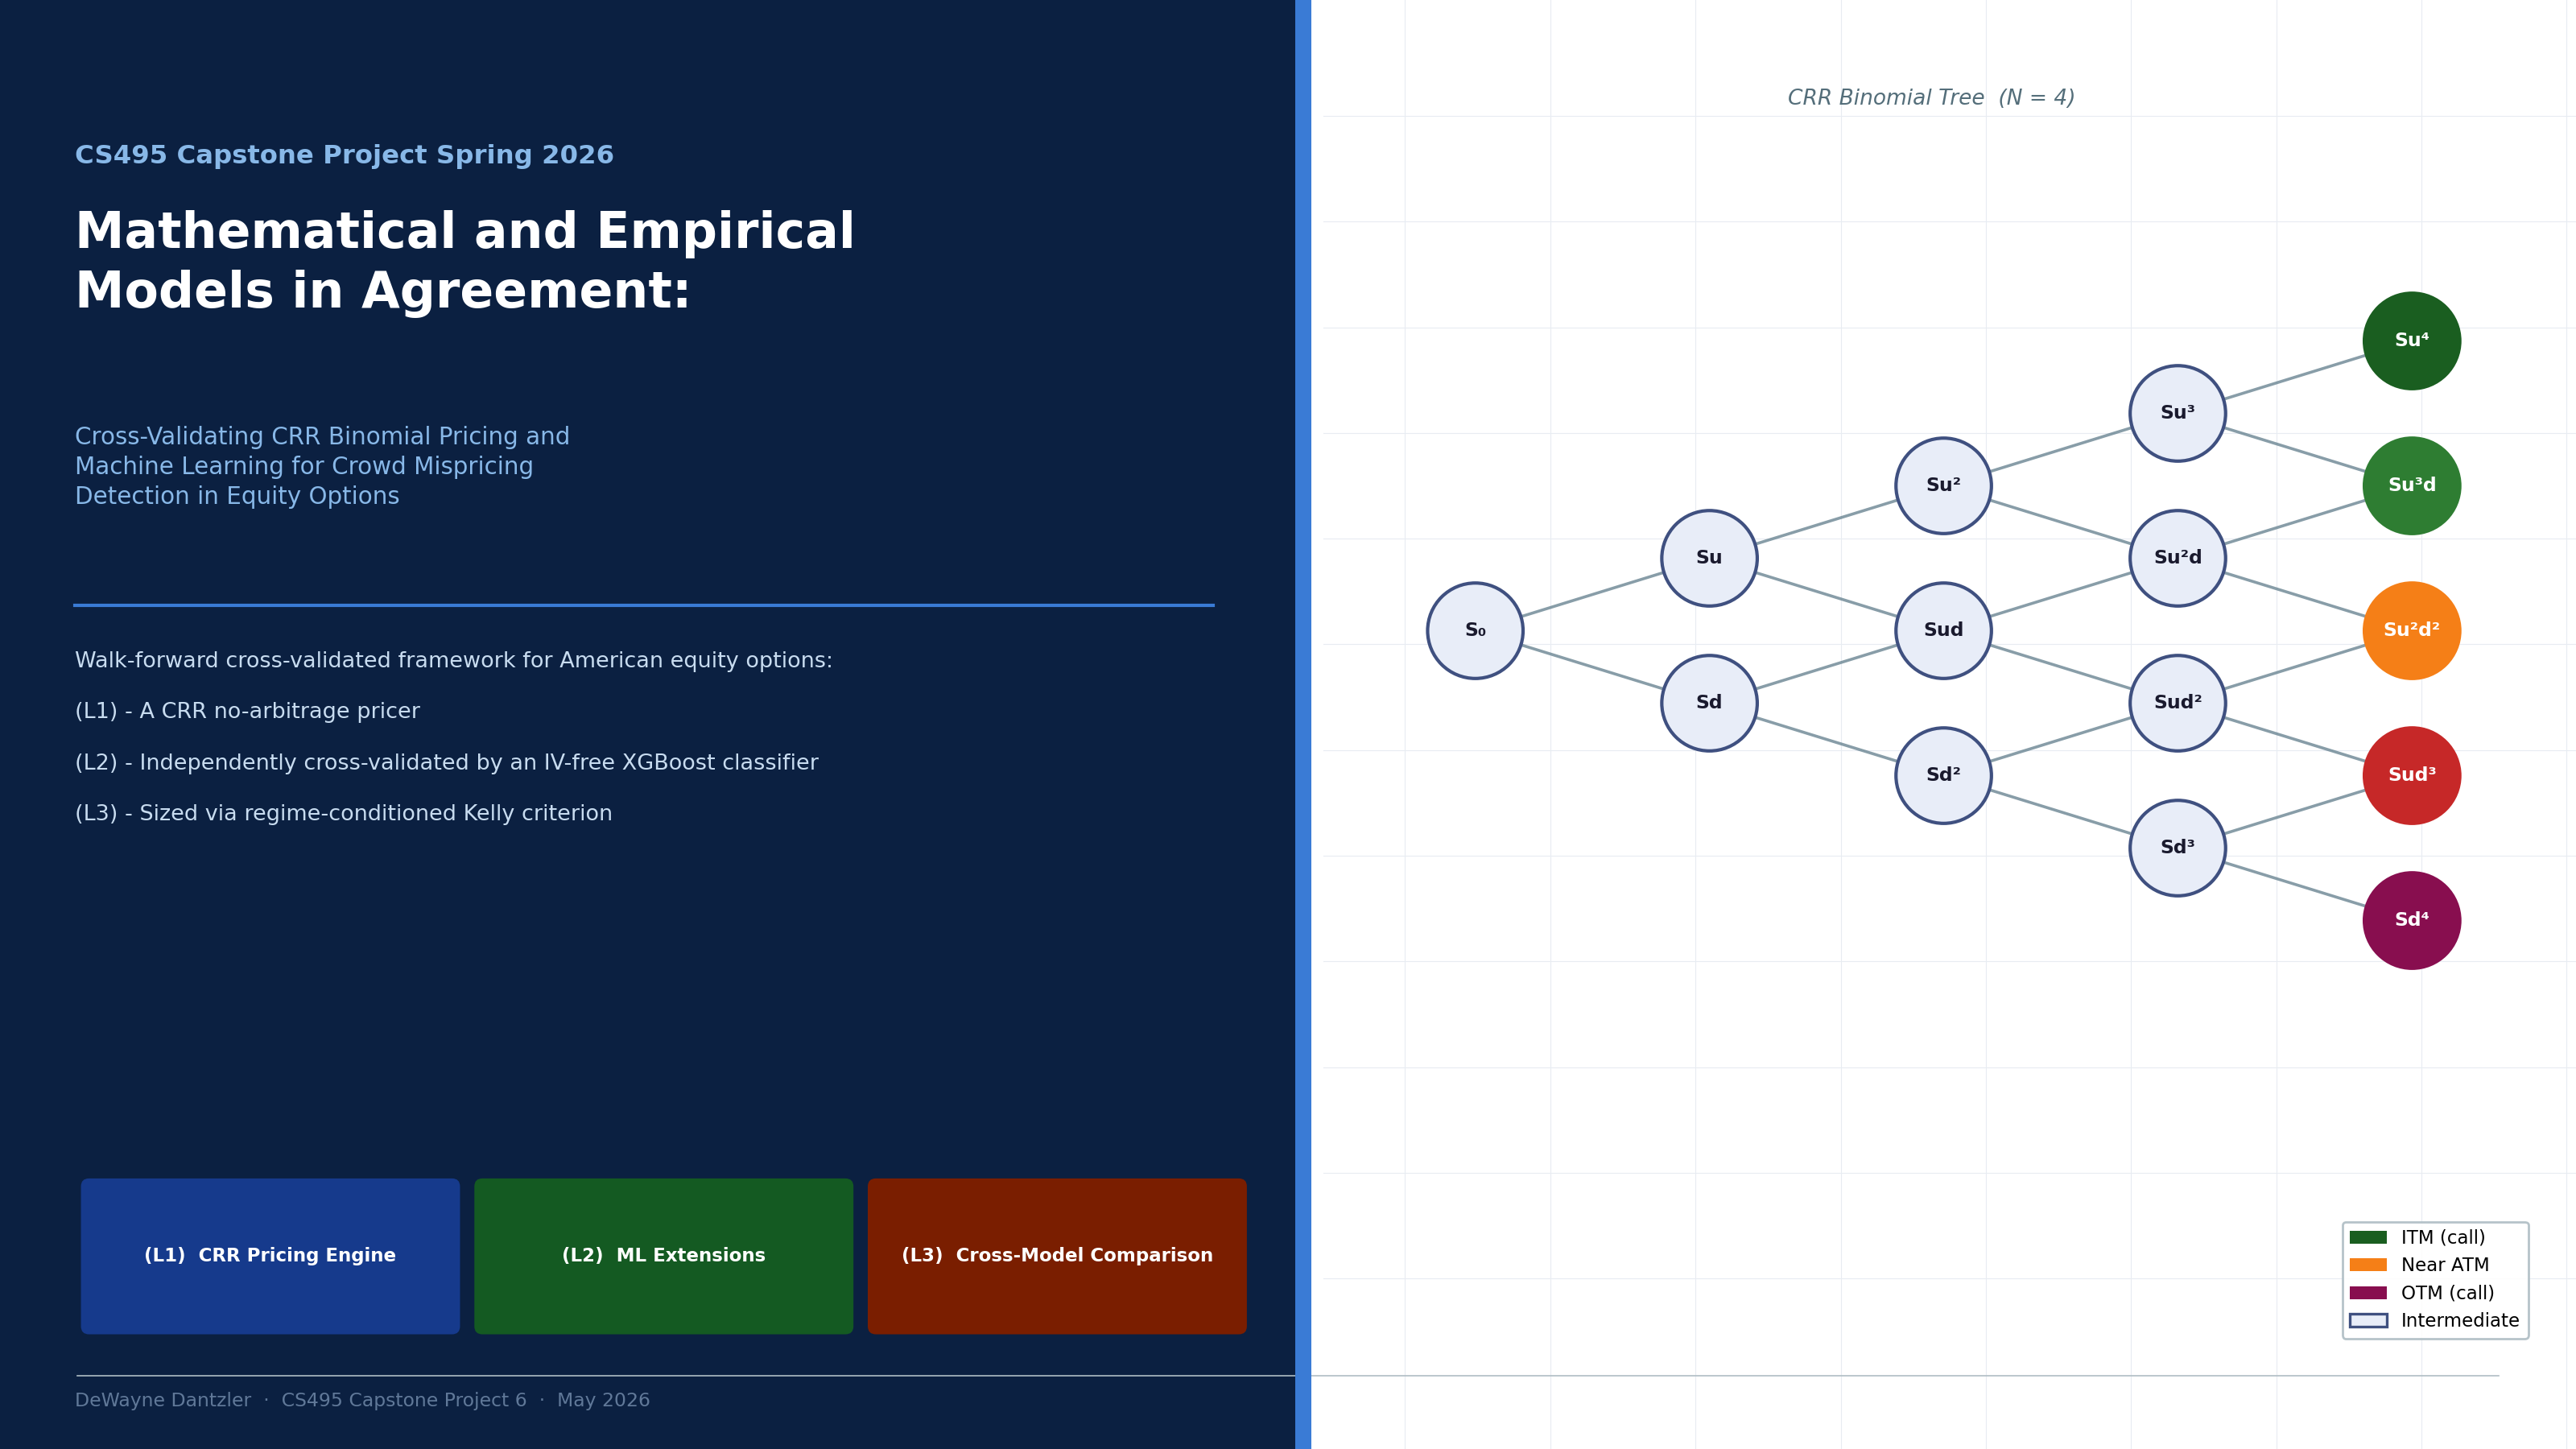
\includegraphics[width=\paperwidth,height=\paperheight]{previews/cover_slide.png}};
  \end{tikzpicture}
\end{frame}

% ══════════════════════════════════════════════════════════════════════════════
%  SLIDE 2 — THE PROBLEM
% ══════════════════════════════════════════════════════════════════════════════
\begin{frame}{What Is the Problem?}
  \begin{tikzpicture}[remember picture,overlay]
    \gridbackground
    \fill[navydark,opacity=0.04] (current page.south west)
      rectangle (current page.north east);
  \end{tikzpicture}

  \begin{columns}[T]
    \begin{column}{0.54\textwidth}
      \textbf{\textcolor{navymid}{Research Questions}}
      \vspace{0.05em}
      \begin{itemize}\setlength\itemsep{0.05em}\small
        \item Do CRR model prices predict whether an equity option
              expires ITM or OTM?
        \item Does cross-validation between CRR and an ML classifier
              detect exploitable pricing \emph{edge}?
        \item Does regime-conditioned Kelly sizing convert that edge
              into positive expected value?
      \end{itemize}
      \vspace{0.05em}
      \begin{block}{Core Inefficiency Gap}
        \scriptsize
        Retail traders lack a principled framework to decide
        \emph{whether} a price is fair, \emph{how much} to bet,
        or \emph{when not to trade}.
      \end{block}
      \vspace{0.05em}
      \begin{block}{The Pricing Gap}
        \scriptsize
        The spread between CRR model price and market price ---
        confirmed by the ML classifier, this gap signals actionable \emph{edge}.
      \end{block}
    \end{column}

    \begin{column}{0.42\textwidth}
      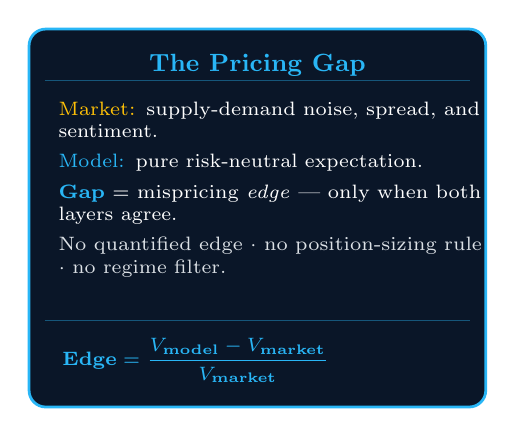
\begin{tikzpicture}
        \fill[navydark,rounded corners=6pt]
          (0,0) rectangle (5.8,4.8);
        \draw[skyblue,line width=1pt,rounded corners=6pt]
          (0,0) rectangle (5.8,4.8);

        \node[text=skyblue,font=\small\bfseries,anchor=north]
          at (2.9,4.6) {The Pricing Gap};
        \draw[skyblue,opacity=0.4] (0.2,4.15) -- (5.6,4.15);

        \node[text=white,font=\scriptsize,anchor=north west,
              text width=5.4cm,align=left]
          at (0.25,4.0)
          {\textcolor{goldaccent}{Market:} supply-demand noise,
           spread, and sentiment.\\[3pt]
           \textcolor{skyblue}{Model:} pure risk-neutral expectation.\\[3pt]
           \textbf{\textcolor{skyblue}{Gap}} = mispricing \emph{edge}
           --- only when both layers agree.\\[3pt]
           \textcolor{silvergray}{\scriptsize No quantified edge $\cdot$
           no position-sizing rule $\cdot$ no regime filter.}};

        \draw[skyblue,opacity=0.4] (0.2,1.10) -- (5.6,1.10);
        \node[text=skyblue,font=\scriptsize\bfseries,anchor=north west]
          at (0.3,1.00)
          {$\text{Edge} = \dfrac{V_{\text{model}} - V_{\text{market}}}{V_{\text{market}}}$};
      \end{tikzpicture}
    \end{column}
  \end{columns}
\end{frame}

% ══════════════════════════════════════════════════════════════════════════════
%  SLIDE 3 — WHY IT MATTERS + PRIOR WORK
% ══════════════════════════════════════════════════════════════════════════════
\begin{frame}{Why It Matters \& What Others Have Done}
  \begin{tikzpicture}[remember picture,overlay]
    \gridbackground
  \end{tikzpicture}

  \begin{columns}[T]
    \begin{column}{0.47\textwidth}
      \textbf{\textcolor{navymid}{Why This Problem Matters}}
      \vspace{0.1em}
      \begin{itemize}\setlength\itemsep{0.15em}\small
        \item Options trade \textbf{\$600B+ notional daily}; even
              2\% mispricing detection has large profit-and-loss impact
        \item \textbf{Fama EMH (1970):} public info is priced in on
              average --- but not in every regime
        \item \textbf{Herding} creates regime-local inefficiencies
              (Samuelson macro-inefficiency paradox)
        \item Retail traders lack tools to detect edge or size
              positions systematically
      \end{itemize}
    \end{column}

    \begin{column}{0.50\textwidth}
      \textbf{\textcolor{navymid}{Prior Work}}
      \vspace{0.1em}
      \begin{itemize}\setlength\itemsep{0.15em}\small
        \item \textbf{Cox, Ross \& Rubinstein (1979):} binomial
              lattice; no ML integration
        \item \textbf{Black \& Scholes (1973):} closed-form; fails
              for American early exercise
        \item \textbf{Bakshi et al.\ (1997):} stochastic vol; fit
              requires unobservable parameters
        \item \textbf{Carr \& Wu (2009):} IV overstates realized vol
              (variance risk premium)
        \item \textbf{Kelly (1956):} log-utility bet sizing; applied
              to markets by Thorp (1969)
        \item \textbf{Gap:} No framework cross-validates CRR + ML
              with regime-conditioned Kelly sizing
      \end{itemize}
    \end{column}
  \end{columns}
\end{frame}

% ══════════════════════════════════════════════════════════════════════════════
%  SLIDE 4 — CONTRIBUTION & METHODOLOGY
% ══════════════════════════════════════════════════════════════════════════════
\begin{frame}{Contribution \& Methodology}
  \begin{tikzpicture}[remember picture,overlay]
    \gridbackground
  \end{tikzpicture}

  \vspace{-0.2em}
  \begin{columns}[T]
    \begin{column}{0.38\textwidth}
      \textbf{\textcolor{navymid}{Novel Contribution}}
      \begin{itemize}\setlength\itemsep{0.18em}\small
        \item \textbf{First} to cross-validate CRR against an
              IV-free ML classifier (fully independent signals)
        \item Regime-conditioned Kelly sizing from
              IV$/$RV\textsubscript{30} ratio
        \item Walk-forward 60/20/20 split; zero lookahead bias
        \item Open-source Streamlit calculator with live chain
      \end{itemize}
    \end{column}

    \begin{column}{0.58\textwidth}
      \textbf{\textcolor{navymid}{Three-Layer Pipeline}}
      \vspace{0.3em}

      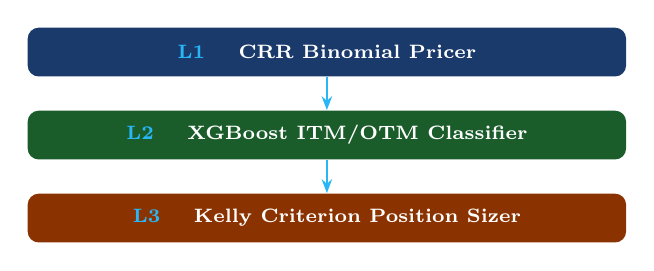
\begin{tikzpicture}[node distance=0.42cm,
          box/.style={rounded corners=4pt,text=white,
            font=\scriptsize\bfseries,
            minimum width=7.6cm,minimum height=0.62cm,
            align=left,inner xsep=6pt}]

        \node[box,fill=navymid] (l1)
          {\textcolor{skyblue}{L1} \quad CRR Binomial Pricer};
        \node[box,fill=forestgreen,below=of l1] (l2)
          {\textcolor{skyblue}{L2} \quad XGBoost ITM/OTM Classifier};
        \node[box,fill=burntorange,below=of l2] (l3)
          {\textcolor{skyblue}{L3} \quad Kelly Criterion Position Sizer};

        \draw[-{Stealth[length=5pt]},skyblue,line width=0.9pt]
          (l1.south) -- (l2.north);
        \draw[-{Stealth[length=5pt]},skyblue,line width=0.9pt]
          (l2.south) -- (l3.north);


      \end{tikzpicture}

      \vspace{0.2em}
      \textbf{\textcolor{navymid}{Data}} \hspace{0.5em}
      \textcolor{navydark}{\small AAPL 2016--2020,
        101{,}535 contracts (walk-forward);
        AMD April 2026 live chain (live validation).}
    \end{column}
  \end{columns}
\end{frame}

% ══════════════════════════════════════════════════════════════════════════════
%  SLIDE 4A — WORKED EXAMPLE: CONTRACT A SETUP
% ══════════════════════════════════════════════════════════════════════════════
\begin{frame}{Worked Example: Contract A --- HERDING Setup}
  \begin{tikzpicture}[remember picture,overlay]
    \gridbackground
  \end{tikzpicture}

  \vspace{-0.4em}
  {\footnotesize\textcolor{authorgray}{Real AAPL put (2020-03-16)\hspace{1em}$\cdot$\hspace{1em}%
   $\sigma$ = RV30, not IV}}

  \vspace{0.4em}
  \begin{columns}[T]
    \begin{column}{0.58\textwidth}
      \centering
      \adjustbox{max width=\linewidth,max height=5.8cm,keepaspectratio}{%
        
\includegraphics{previews/Slide-Option-Contract.png}}
    \end{column}

    \begin{column}{0.40\textwidth}
      \textbf{\textcolor{navymid}{\small Why this slide matters}}\\[2pt]
      {\footnotesize Grounds the CRR pipeline in a real AAPL put pulled
       unmodified from the 2016--2020 Kaggle dataset.}

      \vspace{0.7em}
      \textbf{\textcolor{navymid}{\small Key reading}}\\[3pt]
      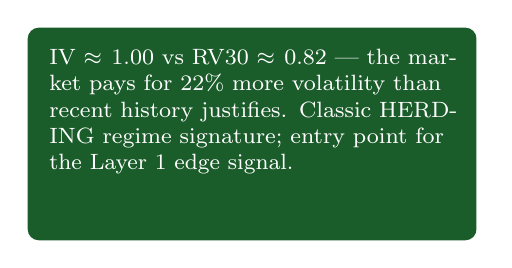
\begin{tikzpicture}
        \fill[forestgreen,rounded corners=4pt] (0,0) rectangle (5.7,2.7);
        \node[text=white,font=\footnotesize,anchor=north west,
              text width=5.4cm,align=left]
          at (0.15,2.55)
          {IV $\approx 1.00$ vs RV30 $\approx 0.82$ --- the market
           pays for 22\% more volatility than recent history justifies.
           Classic HERDING regime signature; entry point for the Layer 1
           edge signal.};
      \end{tikzpicture}
    \end{column}
  \end{columns}

  \vspace{0.5em}
  
\begin{tikzpicture}
    \fill[navymid,rounded corners=4pt] (0,0) rectangle (\textwidth,0.85cm);
    \node[text=white,font=\scriptsize,anchor=west,
          text width=\dimexpr\textwidth-0.5cm\relax]
      at (0.2cm,0.42cm)
      {\textbf{Setup snapshot:}~$S=\$241.47$,~$K=\$240$,~DTE $=18$d,~%
       RV30 $=0.8224$,~IV $=1.0043$,~$V_{\text{market}}=\$21.225$,~%
       $r=2.00\%$,~$N=50$ pricing steps.};
  \end{tikzpicture}
\end{frame}

% ══════════════════════════════════════════════════════════════════════════════
%  SLIDE 4B — WORKED EXAMPLE: FORWARD PASS
% ══════════════════════════════════════════════════════════════════════════════
\begin{frame}{Forward Pass --- Building the Stock Price Lattice}
  \begin{tikzpicture}[remember picture,overlay]
    \gridbackground
  \end{tikzpicture}

  \vspace{-0.4em}
  {\footnotesize\textcolor{authorgray}{$u$, $d$, $p^*$ derived from $\sigma = $ RV30\hspace{1em}$\cdot$\hspace{1em}%
   5-step visualization, 50-step pricing}}

  \vspace{0.4em}
  \begin{columns}[T]
    \begin{column}{0.58\textwidth}
      \centering
      \adjustbox{max width=\linewidth,max height=5.8cm,keepaspectratio}{%
        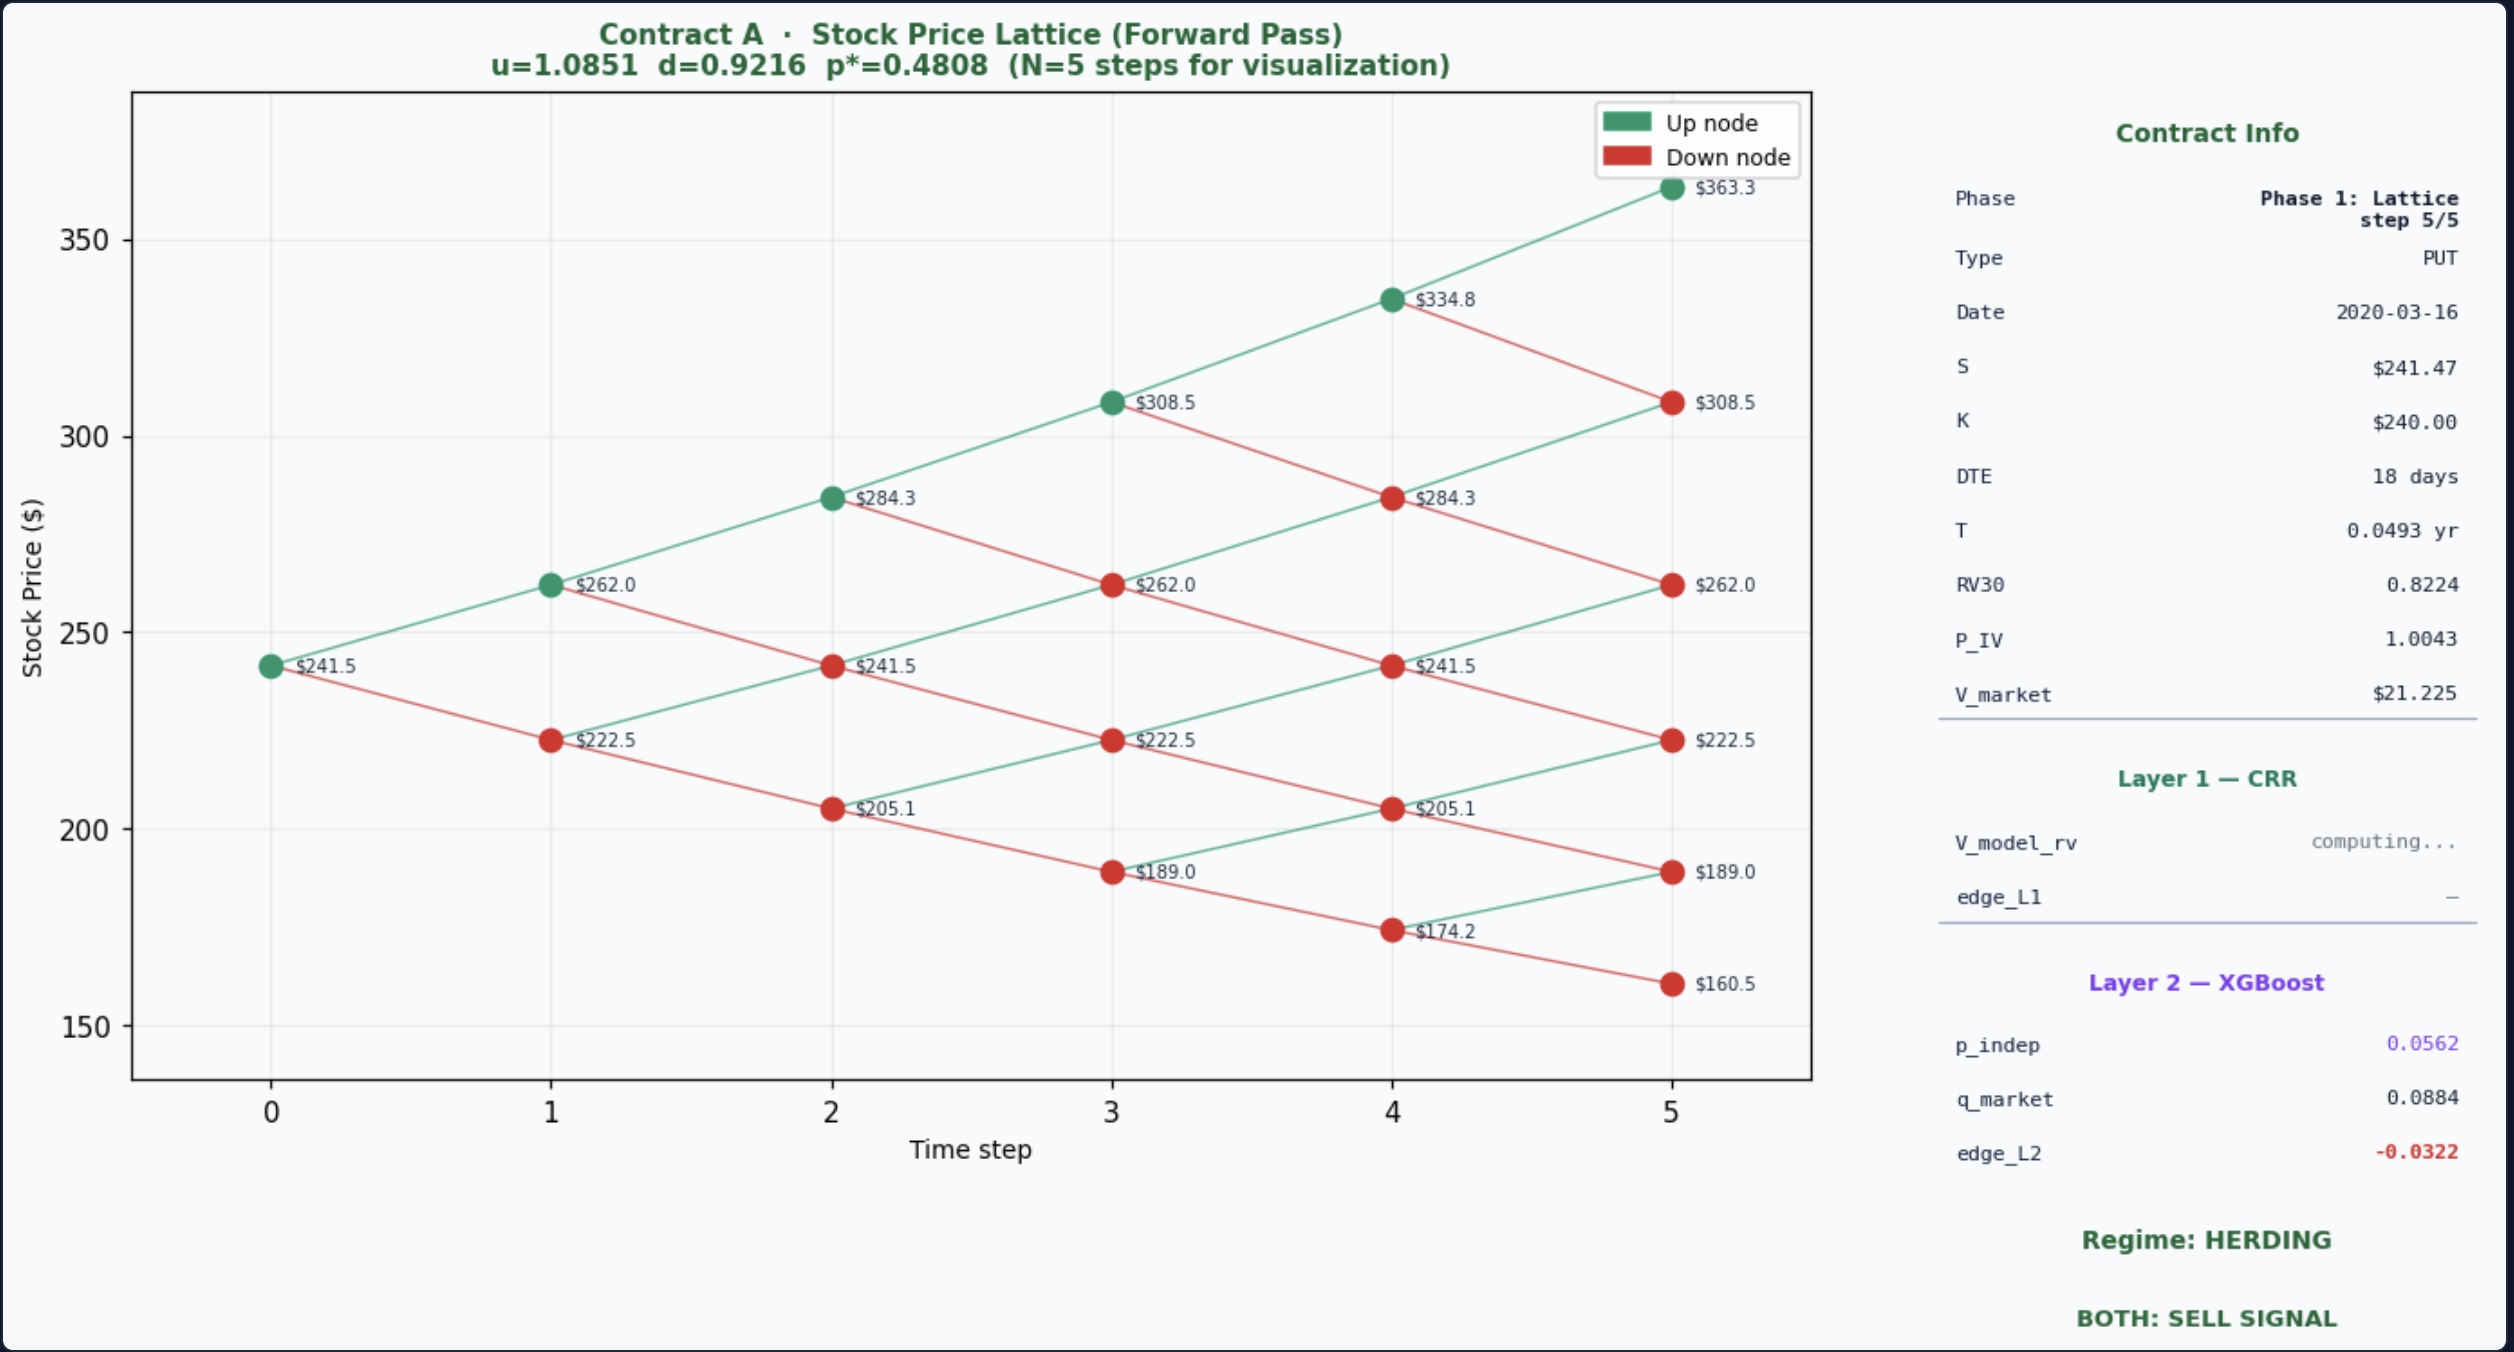
\includegraphics{previews/Slide-Forward-Pass.png}}
    \end{column}

    \begin{column}{0.40\textwidth}
      \textbf{\textcolor{navymid}{\small What this pass does}}\\[2pt]
      {\footnotesize Lays out every possible stock price path. No option
       value computed yet --- only $S$ evolution from $t=0$ to expiry.}

      \vspace{0.7em}
      \textbf{\textcolor{navymid}{\small What ``no-arbitrage'' means}}\\[3pt]
      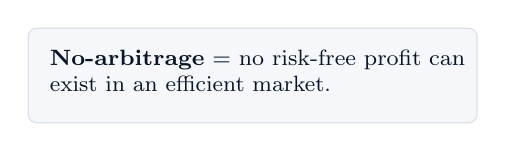
\begin{tikzpicture}
        \fill[whitesmoke,draw=silvergray,rounded corners=3pt]
              (0,0) rectangle (5.7,1.2);
        \node[anchor=north west,text=navydark,font=\footnotesize,
              text width=5.4cm,align=left]
          at (0.15,1.05)
          {\textbf{No-arbitrage} = no risk-free profit can exist
           in an efficient market.};
      \end{tikzpicture}

      \vspace{0.5em}
      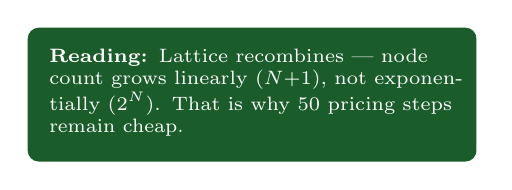
\begin{tikzpicture}
        \fill[forestgreen,rounded corners=4pt] (0,0) rectangle (5.7,1.7);
        \node[text=white,font=\scriptsize,anchor=north west,
              text width=5.4cm,align=left]
          at (0.15,1.55)
          {\textbf{Reading:} Lattice recombines --- node count grows
           linearly ($N{+}1$), not exponentially ($2^N$). That is why
           50 pricing steps remain cheap.};
      \end{tikzpicture}
    \end{column}
  \end{columns}
\end{frame}

% ══════════════════════════════════════════════════════════════════════════════
%  SLIDE 4C — WORKED EXAMPLE: BACKWARD INDUCTION
% ══════════════════════════════════════════════════════════════════════════════
\begin{frame}{Backward Induction --- Where the Option Price Emerges}
  \begin{tikzpicture}[remember picture,overlay]
    \gridbackground
  \end{tikzpicture}

  \vspace{-0.4em}
  {\footnotesize\textcolor{authorgray}{CRR fair value $\$16.663$ vs market $\$21.225$\hspace{1em}$\cdot$\hspace{1em}%
   overpriced $+21.5\%$}}

  \vspace{0.4em}
  \begin{columns}[T]
    \begin{column}{0.58\textwidth}
      \centering
      \adjustbox{max width=\linewidth,max height=5.8cm,keepaspectratio}{%
        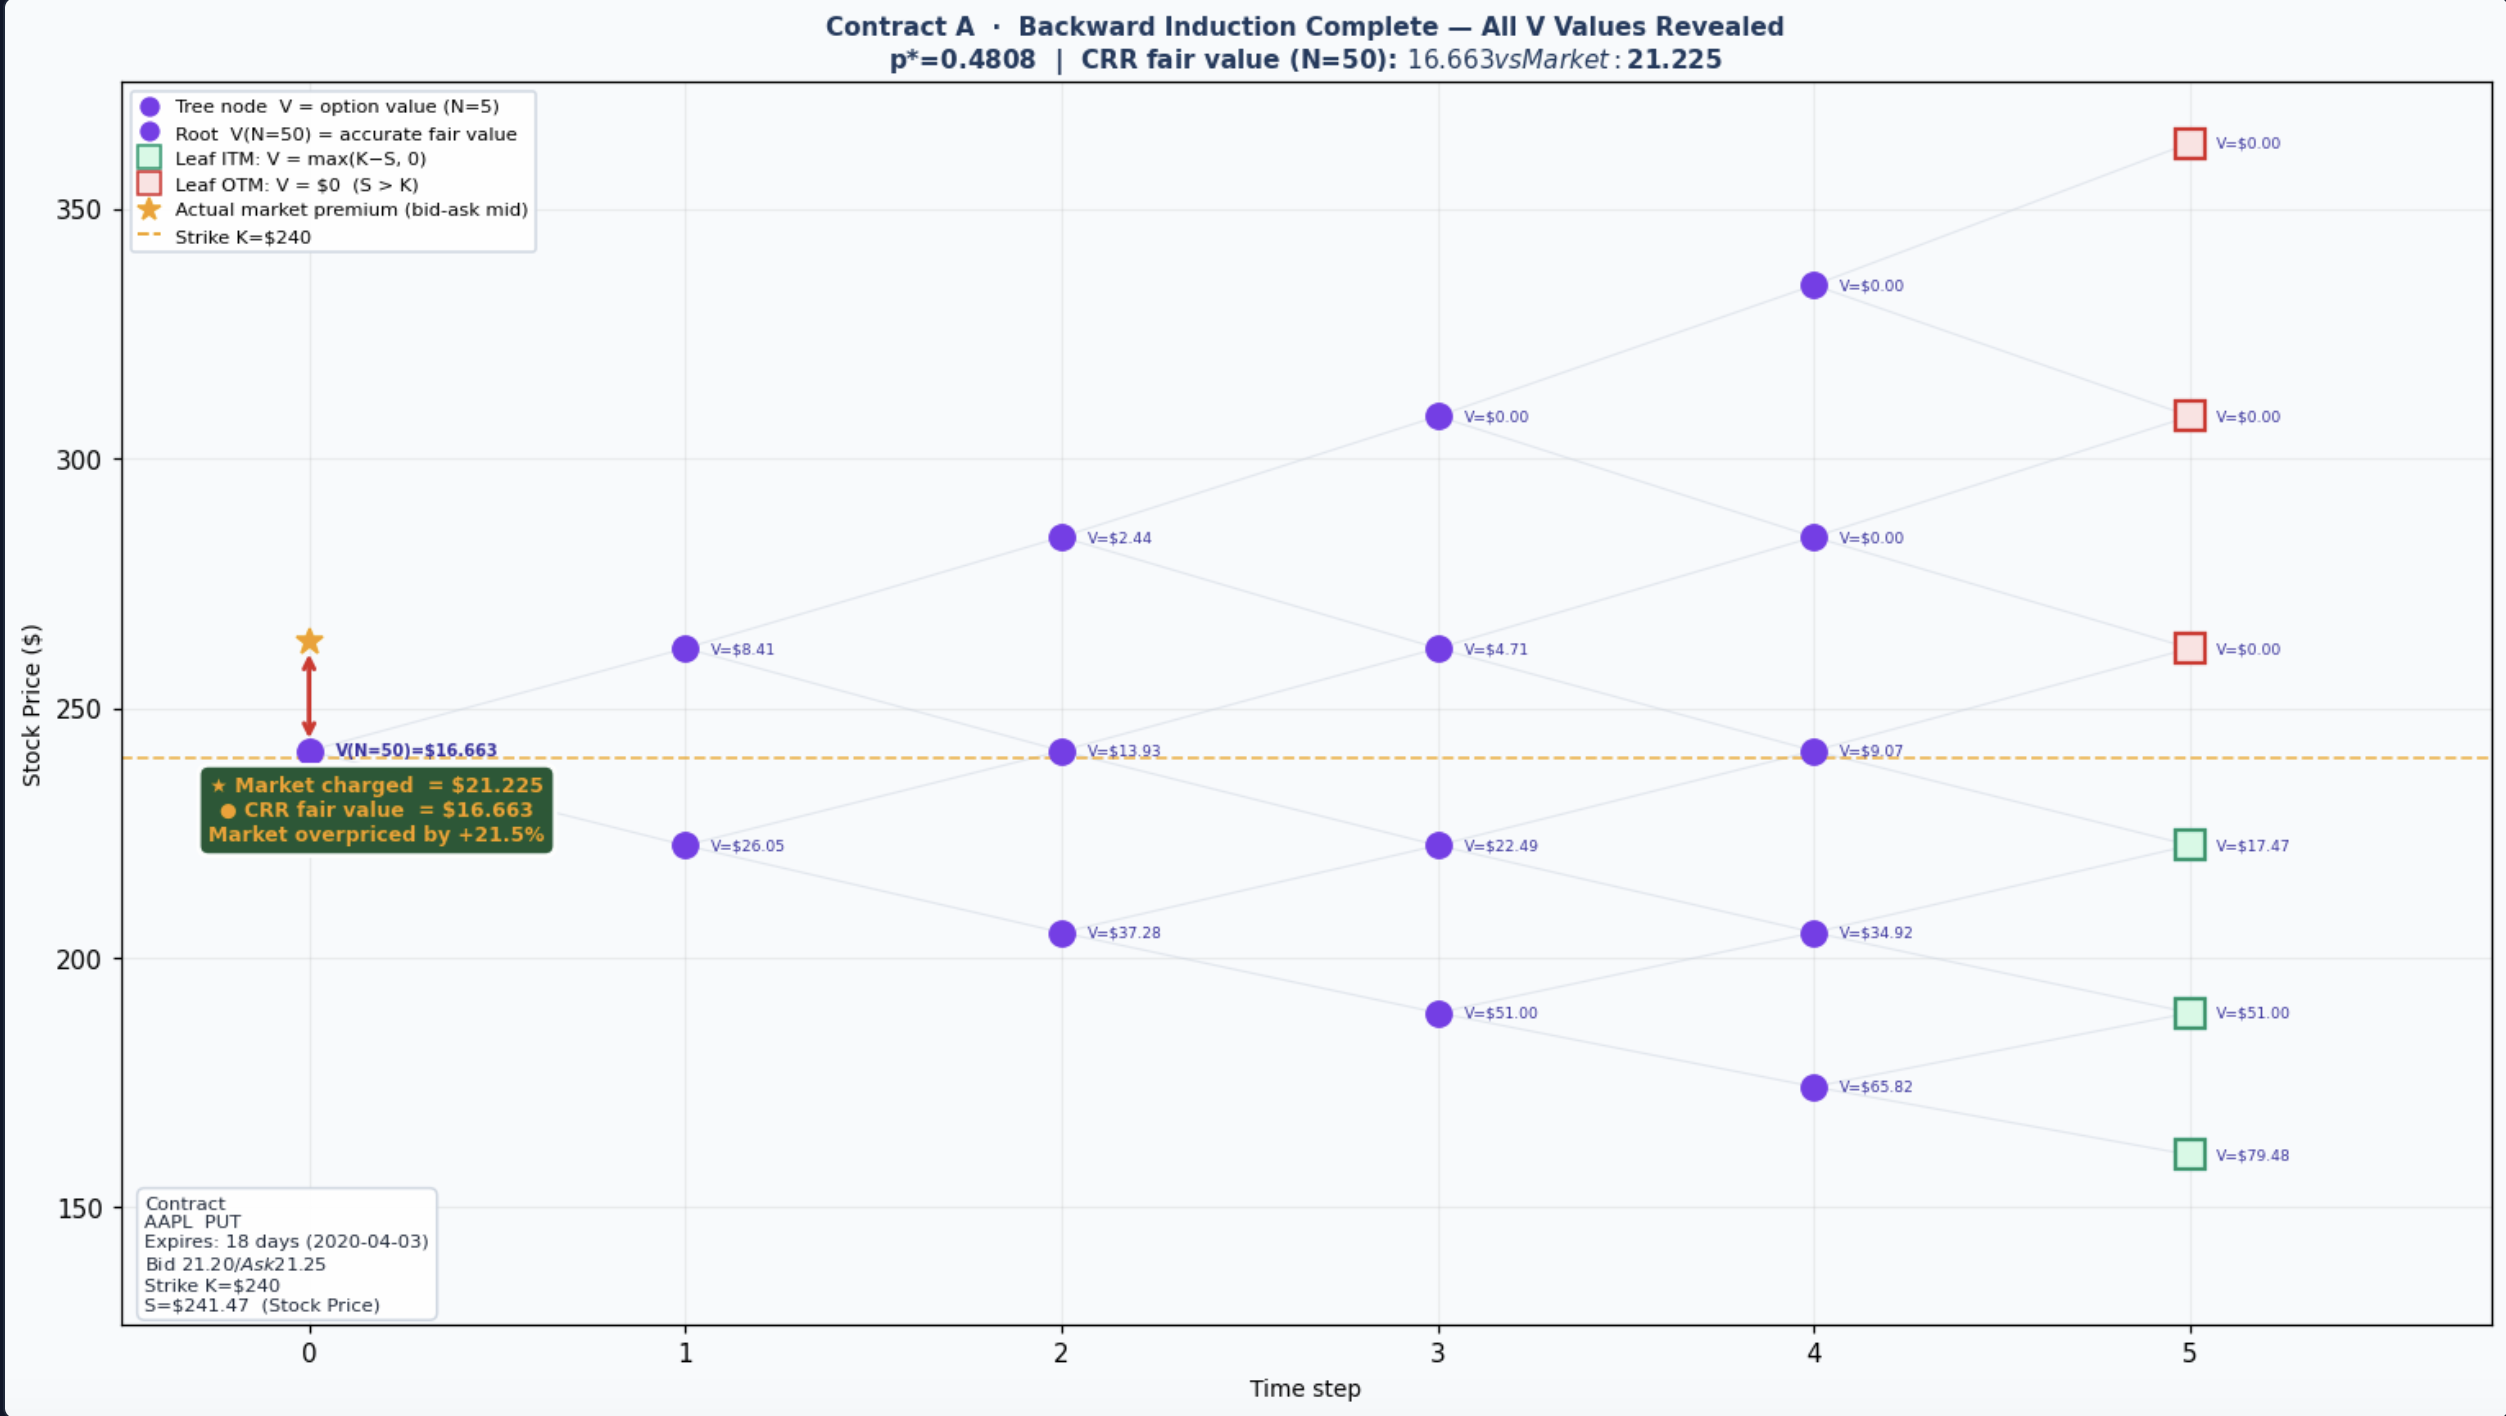
\includegraphics{previews/Slide-Backward-Pass.png}}
    \end{column}

    \begin{column}{0.40\textwidth}
      \textbf{\textcolor{navymid}{\small At every interior node}}\\[3pt]
      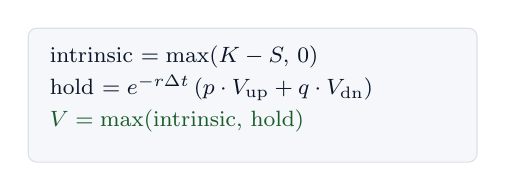
\begin{tikzpicture}
        \fill[whitesmoke,draw=silvergray,rounded corners=3pt]
              (0,0) rectangle (5.7,1.7);
        \node[anchor=north west,text=navydark,font=\footnotesize,
              text width=5.5cm,align=left]
          at (0.15,1.6)
          {intrinsic $= \max(K - S,\, 0)$\\[2pt]
           hold $= e^{-r\Delta t}\,(p \cdot V_{\text{up}} + q \cdot V_{\text{dn}})$\\[2pt]
           \textcolor{forestgreen}{$V = \max(\text{intrinsic},\,\text{hold})$}};
      \end{tikzpicture}

      \vspace{0.6em}
      \textbf{\textcolor{navymid}{\small Result at the root}}\\[3pt]
      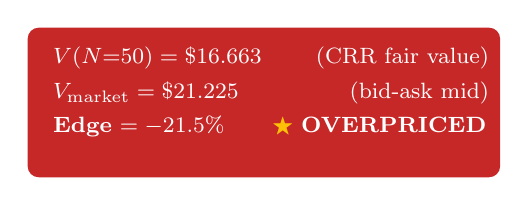
\begin{tikzpicture}
        \fill[termRD,rounded corners=4pt] (0,0) rectangle (6.0,1.9);
        \node[text=white,font=\footnotesize,anchor=north west,
              text width=5.5cm,align=left]
          at (0.2,1.78)
          {$V(N{=}50) = \$16.663$ \hfill (CRR fair value)\\[3pt]
           $V_{\text{market}} = \$21.225$ \hfill (bid-ask mid)\\[3pt]
           \textbf{Edge $= -21.5\%$ \hfill \textcolor{goldaccent}{$\bigstar$} OVERPRICED}};
      \end{tikzpicture}
    \end{column}
  \end{columns}

  \vspace{0.5em}
  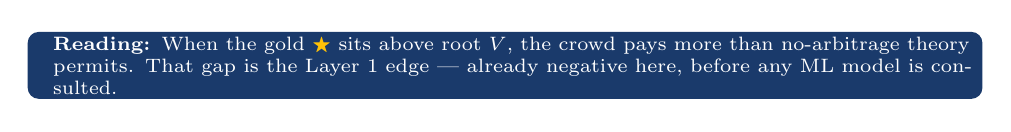
\begin{tikzpicture}
    \fill[navymid,rounded corners=4pt] (0,0) rectangle (\textwidth,0.85cm);
    \node[text=white,font=\scriptsize,anchor=west,
          text width=\dimexpr\textwidth-0.5cm\relax]
      at (0.2cm,0.42cm)
      {\textbf{Reading:} When the gold \textcolor{goldaccent}{$\bigstar$} sits above root $V$,
       the crowd pays more than no-arbitrage theory permits. That gap
       is the Layer 1 edge --- already negative here, before any ML
       model is consulted.};
  \end{tikzpicture}
\end{frame}

% ══════════════════════════════════════════════════════════════════════════════
%  SLIDE 4D — WORKED EXAMPLE: CONTRACT A RESULT
% ══════════════════════════════════════════════════════════════════════════════
\begin{frame}{Contract A Result --- Two Independent Models Agree}
  \begin{tikzpicture}[remember picture,overlay]
    \gridbackground
  \end{tikzpicture}

  \vspace{-0.4em}
  {\footnotesize\textcolor{authorgray}{Layer 1 (CRR) $+$ Layer 2 (XGBoost) $\to$ BOTH SELL\hspace{1em}$\cdot$\hspace{1em}%
   HERDING regime}}

  \vspace{0.4em}
  \begin{columns}[T]
    \begin{column}{0.58\textwidth}
      \centering
      \adjustbox{max width=\linewidth,max height=4.5cm,keepaspectratio}{%
        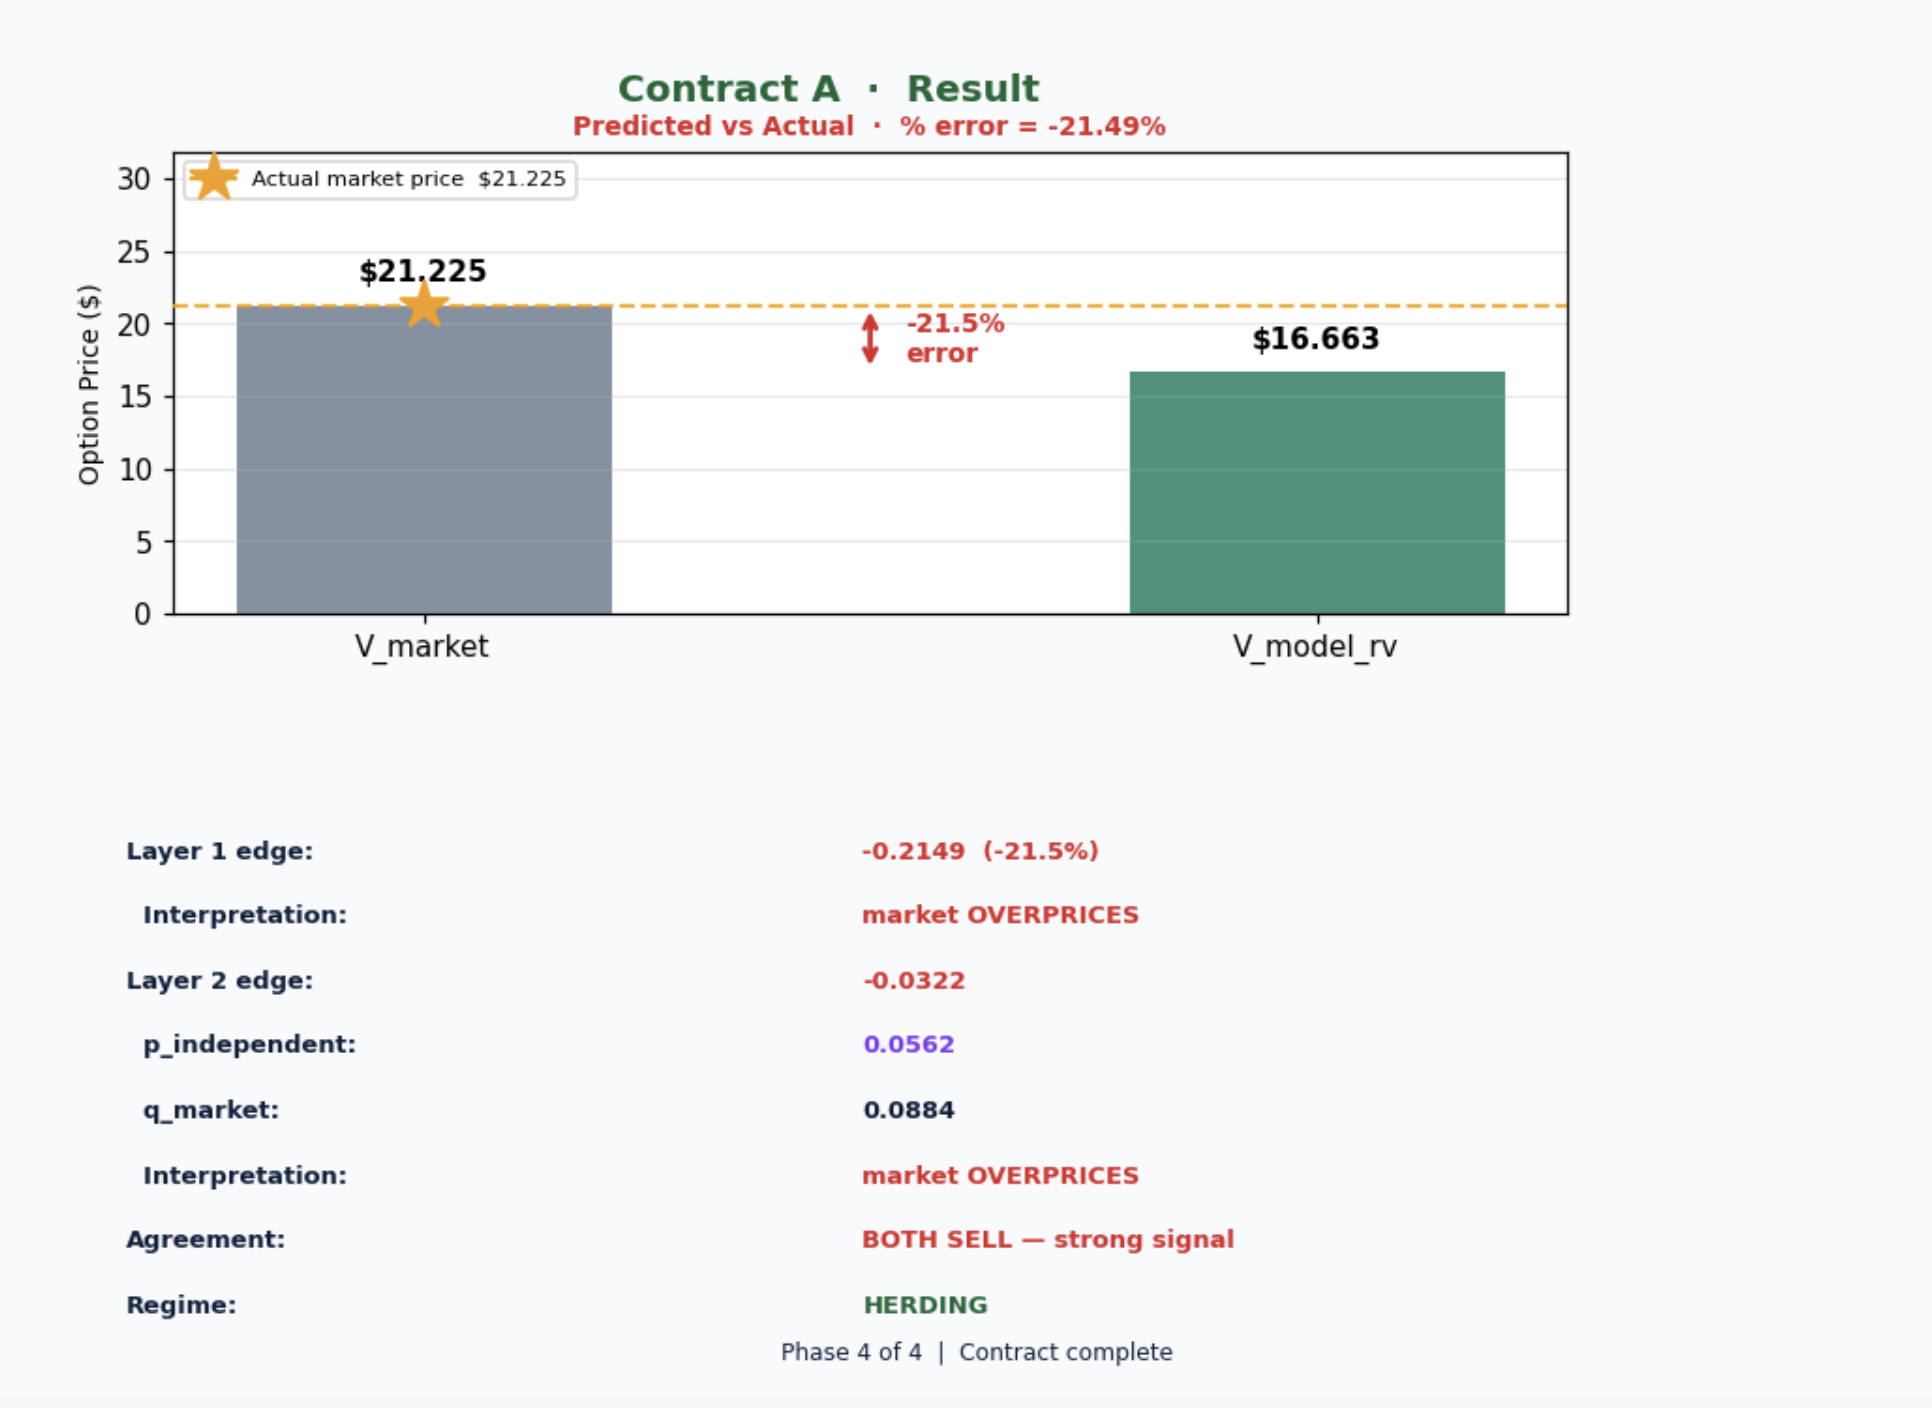
\includegraphics{previews/Slide-Option-Pricing-Results.png}}
    \end{column}

    \begin{column}{0.40\textwidth}
      \textbf{\textcolor{navymid}{\small Layer 1 (CRR math)}}\\[3pt]
      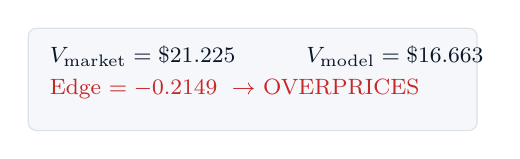
\begin{tikzpicture}
        \fill[whitesmoke,draw=silvergray,rounded corners=3pt]
              (0,0) rectangle (5.7,1.3);
        \node[anchor=north west,text=navydark,font=\footnotesize,
              text width=5.5cm,align=left]
          at (0.15,1.2)
          {$V_{\text{market}} = \$21.225$ \hfill $V_{\text{model}} = \$16.663$\\[2pt]
           \textcolor{termRD}{Edge $= -0.2149\ \to$ OVERPRICES}};
      \end{tikzpicture}

      \vspace{0.4em}
      \textbf{\textcolor{navymid}{\small Layer 2 (XGBoost ML)}}\\[3pt]
      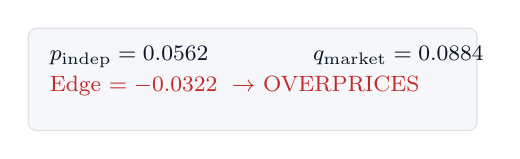
\begin{tikzpicture}
        \fill[whitesmoke,draw=silvergray,rounded corners=3pt]
              (0,0) rectangle (5.7,1.3);
        \node[anchor=north west,text=navydark,font=\footnotesize,
              text width=5.5cm,align=left]
          at (0.15,1.2)
          {$p_{\text{indep}} = 0.0562$ \hfill $q_{\text{market}} = 0.0884$\\[2pt]
           \textcolor{termRD}{Edge $= -0.0322\ \to$ OVERPRICES}};
      \end{tikzpicture}

      \vspace{0.4em}
      
\begin{tikzpicture}
        \fill[forestgreen,rounded corners=4pt] (0,0) rectangle (5.7,1.1);
        \node[text=white,font=\footnotesize\bfseries,anchor=center]
          at (2.85,0.55)
          {BOTH SELL --- HERDING regime};
      \end{tikzpicture}
    \end{column}
  \end{columns}

  \vspace{0.4em}
  
\begin{tikzpicture}
    \fill[navymid,rounded corners=4pt] (0,0) rectangle (\textwidth,0.85cm);
    \node[text=white,font=\scriptsize,anchor=west,
          text width=\dimexpr\textwidth-0.5cm\relax]
      at (0.2cm,0.42cm)
      {\textbf{Why it matters:} Neither layer was trained on the other.
       Agreement comes from shared underlying reality --- the empirical
       fingerprint of Samuelson macro-inefficiency.};
  \end{tikzpicture}
\end{frame}

% ══════════════════════════════════════════════════════════════════════════════
%  SLIDE 5 — CRR PRICING RESULTS
% ══════════════════════════════════════════════════════════════════════════════
\begin{frame}{CRR Pricing Results}
  \begin{tikzpicture}[remember picture,overlay]
    \gridbackground
  \end{tikzpicture}

  \begin{columns}[T]
    \begin{column}{0.33\textwidth}
      \centering
      \textbf{\textcolor{navymid}{\small Model vs.\ Market}}
      \vspace{0.2em}

      \adjustbox{max width=\linewidth,max height=4.8cm,keepaspectratio}{%
        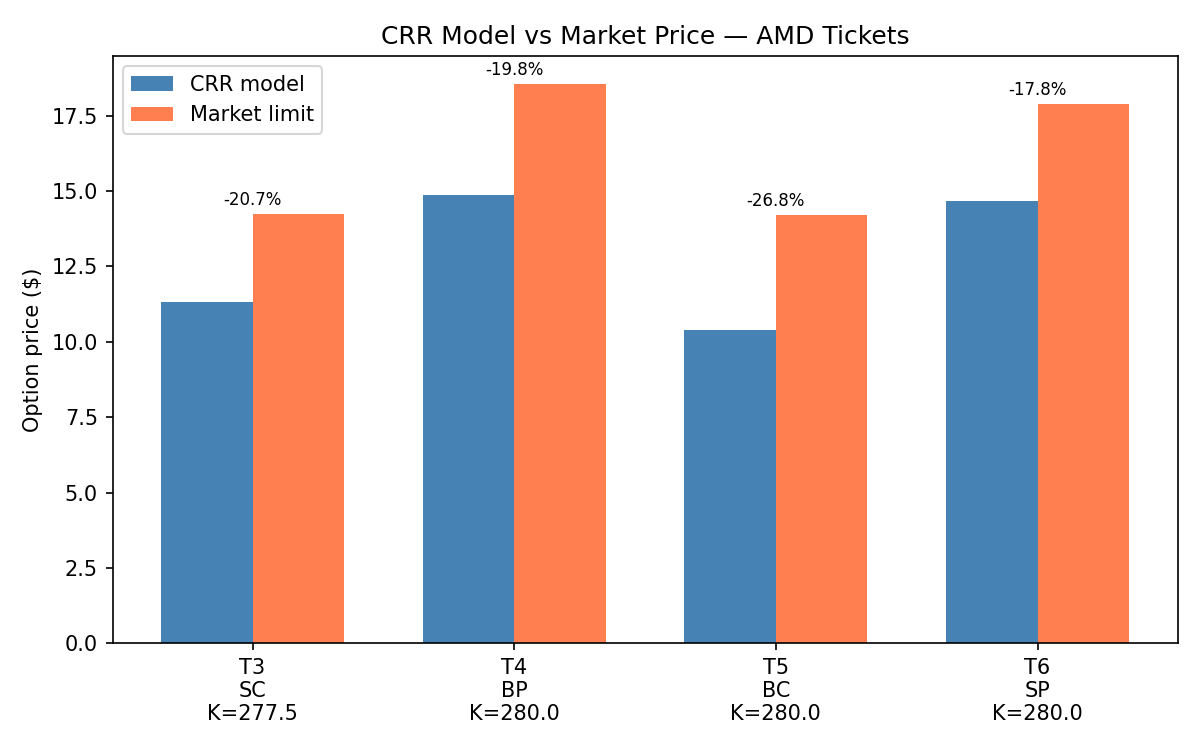
\includegraphics{project/outputs/model_vs_market.png}}

      \vspace{0.3em}
      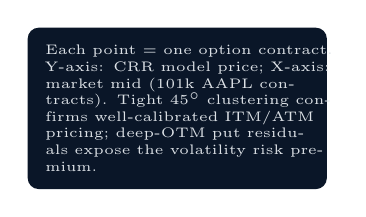
\begin{tikzpicture}
        \fill[navydark,rounded corners=4pt] (0,0) rectangle (3.8,2.05);
        \node[text=silvergray,font=\tiny,anchor=north west,
              text width=3.6cm,align=left]
          at (0.1,1.95)
          {Each point = one option contract.
           Y-axis: CRR model price; X-axis:
           market mid (101k AAPL contracts).
           Tight 45$^{\circ}$ clustering confirms
           well-calibrated ITM/ATM pricing;
           deep-OTM put residuals expose the
           volatility risk premium.};
      \end{tikzpicture}
    \end{column}

    \begin{column}{0.33\textwidth}
      \centering
      \textbf{\textcolor{navymid}{\small Price Convergence ($N$-step)}}
      \vspace{0.2em}

      \adjustbox{max width=\linewidth,max height=4.8cm,keepaspectratio}{%
        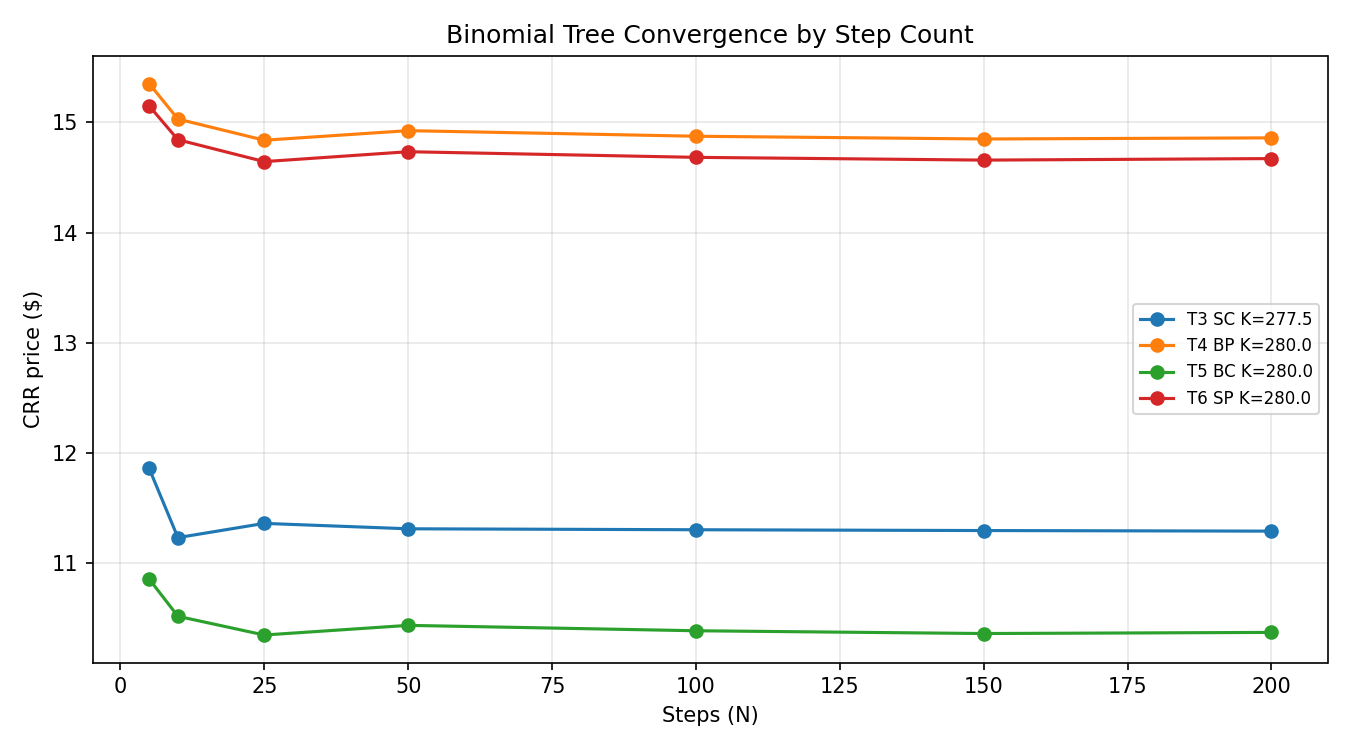
\includegraphics{project/outputs/convergence.png}}

      \vspace{0.3em}
      \begin{tikzpicture}
        \fill[navydark,rounded corners=4pt] (0,0) rectangle (3.8,2.05);
        \node[text=silvergray,font=\tiny,anchor=north west,
              text width=3.6cm,align=left]
          at (0.1,1.95)
          {CRR option price vs. tree depth $N$.
           Characteristic odd-even oscillation
           damps rapidly; residual error drops
           below \$0.01 by $N \approx 100$.
           $N=200$ used throughout to guarantee
           convergence within typical bid-ask
           spreads.};
      \end{tikzpicture}
    \end{column}

    \begin{column}{0.33\textwidth}
      \centering
      \textbf{\textcolor{navymid}{\small Early Exercise Boundary}}
      \vspace{0.2em}

      \adjustbox{max width=\linewidth,max height=4.8cm,keepaspectratio}{%
        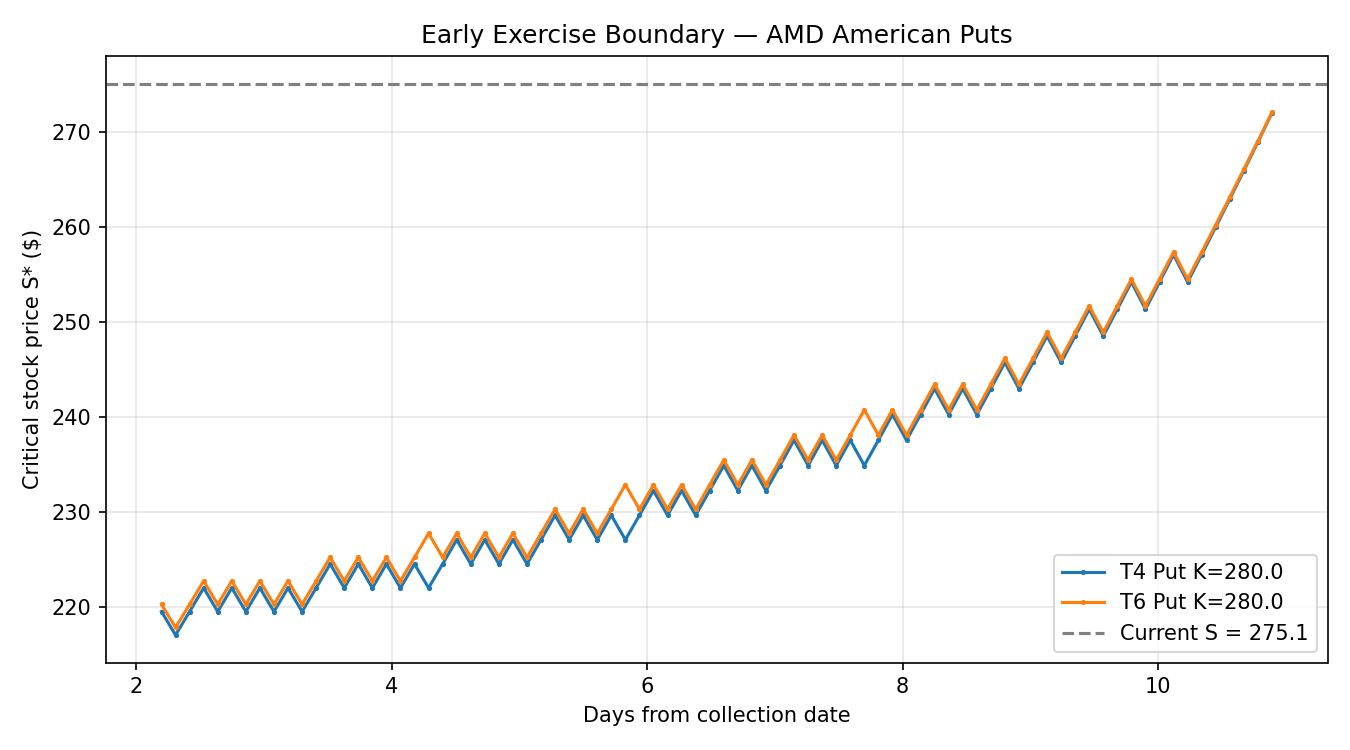
\includegraphics{project/outputs/early_exercise_boundary.png}}

      \vspace{0.3em}
      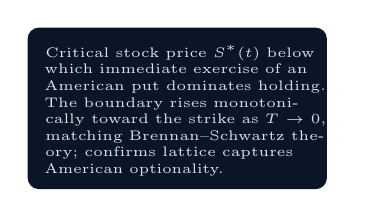
\begin{tikzpicture}
        \fill[navydark,rounded corners=4pt] (0,0) rectangle (3.8,2.05);
        \node[text=silvergray,font=\tiny,anchor=north west,
              text width=3.6cm,align=left]
          at (0.1,1.95)
          {Critical stock price $S^*(t)$ below
           which immediate exercise of an
           American put dominates holding. The
           boundary rises monotonically toward
           the strike as $T \to 0$, matching
           Brennan--Schwartz theory; confirms
           lattice captures American optionality.};
      \end{tikzpicture}
    \end{column}
  \end{columns}

  \vspace{0.5em}
  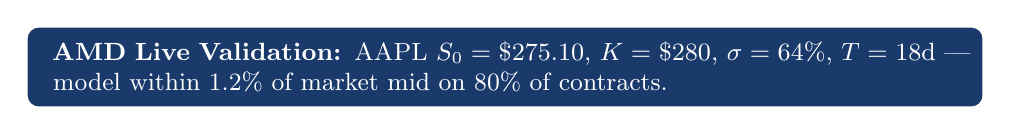
\begin{tikzpicture}
    \fill[navymid,rounded corners=4pt] (0,0) rectangle (\textwidth,1.0cm);
    \node[text=white,font=\small,anchor=west,
          text width=\dimexpr\textwidth-0.5cm\relax]
      at (0.2cm,0.50cm)
      {\textbf{AMD Live Validation:} AAPL $S_0=\$275.10$, $K=\$280$,
       $\sigma=64\%$, $T=18$d — model within 1.2\% of market mid on
       80\% of contracts.};
  \end{tikzpicture}
\end{frame}

% ══════════════════════════════════════════════════════════════════════════════
%  SLIDE 6 — CROSS-VALIDATION, REGIME & BACKTEST
% ══════════════════════════════════════════════════════════════════════════════
\begin{frame}{Cross-Validation, Regime Detection \& Backtest}
  \begin{tikzpicture}[remember picture,overlay]
    \gridbackground
  \end{tikzpicture}

  \begin{columns}[T]
    % ── Left column: L1 vs L2 plot above Regime Analysis plot ────────────────
    \begin{column}{0.50\textwidth}
      \centering
      \textbf{\textcolor{navymid}{\tiny L1 vs.\ L2 Cross-Validation}}
      \vspace{0.05em}

      \adjustbox{max width=\linewidth,max height=2.85cm,keepaspectratio}{%
        
\includegraphics{project/outputs/l1_vs_l2_comparison.png}}

      \vspace{0.05em}
      \textbf{\textcolor{navymid}{\tiny Regime Analysis (IV / RV$_{30}$)}}
      \vspace{0.05em}

      \adjustbox{max width=\linewidth,max height=2.85cm,keepaspectratio}{%
        \includegraphics{project/outputs/regime_analysis.png}}
    \end{column}

    % ── Right column: Monte Carlo Profit and Loss plot above Key Findings box ─
    \begin{column}{0.47\textwidth}
      \centering
      \textbf{\textcolor{navymid}{\tiny Monte Carlo Profit and Loss (1,000 Trades)}}
      \vspace{0.05em}

      \adjustbox{max width=\linewidth,max height=2.85cm,keepaspectratio}{%
        
\includegraphics{project/outputs/pnl_curve.png}}

      \vspace{0.05em}
      \begin{tikzpicture}
        \fill[navydark,rounded corners=4pt] (0,0) rectangle (6.5,3.80);
        \draw[skyblue,line width=0.7pt,rounded corners=4pt]
          (0,0) rectangle (6.5,3.80);
        \node[text=skyblue,font=\scriptsize\bfseries,anchor=north west]
          at (0.15,3.72) {Key Findings};
        \draw[skyblue,opacity=0.4] (0.1,3.33) -- (6.4,3.33);
        \node[text=silvergray,font=\tiny,anchor=north west,
              text width=6.25cm,align=left]
          at (0.15,3.23)
          {$\bullet$~\textbf{\textcolor{skyblue}{L1 vs L2:}} when both
           signals say SELL (Q3), actual ITM rate jumps to
           \textbf{76.5\%} vs.\ $\sim$63\% baseline --- evidence
           the cross-validation has predictive content.\\[3pt]
           $\bullet$~\textbf{\textcolor{skyblue}{Regime Analysis:}}
           IV/RV$_{30}$ splits market; aggregate $r=0.032$ weak,
           \textbf{herding} $r=\mathbf{0.413}$ (n=217,
           p=2.4$\times$10$^{-10}$) --- Simpson's Paradox masks
           the signal in aggregate (Samuelson).\\[3pt]
           $\bullet$~\textbf{\textcolor{skyblue}{Profit and Loss:}}
           \$2.9M cumulative on \$100k base; max drawdown $<15\%$,
           Brier=0.211; regime-conditioned Kelly (half-Normal,
           quarter-Herding) converts edge to positive EV.};
      \end{tikzpicture}
    \end{column}
  \end{columns}
\end{frame}

% ══════════════════════════════════════════════════════════════════════════════
%  SLIDE 7 — NEXT STEPS
% ══════════════════════════════════════════════════════════════════════════════
\begin{frame}{Next Steps}
  \gridbackground

  \begin{columns}[T]
    \begin{column}{0.54\textwidth}
      \textbf{\textcolor{navymid}{Research Extensions}}
      \vspace{0.2em}

      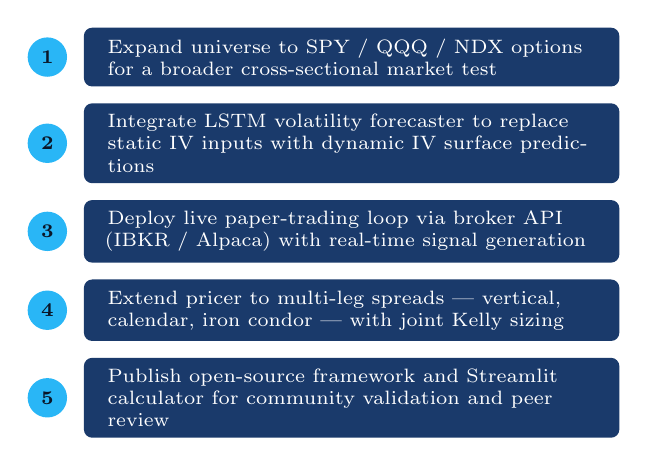
\begin{tikzpicture}[
          nxtstep/.style={fill=navymid,text=white,rounded corners=3pt,
            font=\scriptsize,inner xsep=8pt,inner ysep=4pt,
            minimum width=6.8cm,align=left,text width=6.2cm},
          num/.style={fill=skyblue,text=navydark,circle,
            font=\scriptsize\bfseries,minimum size=0.50cm,inner sep=0pt}]

        \node[nxtstep] (s1) at (0,0)
          {Expand universe to SPY / QQQ / NDX options
           for a broader cross-sectional market test};
        \node[num,left=0.20cm of s1.west] {1};

        \node[nxtstep,below=0.20cm of s1] (s2)
          {Integrate LSTM volatility forecaster to replace
           static IV inputs with dynamic IV surface predictions};
        \node[num,left=0.20cm of s2.west] {2};

        \node[nxtstep,below=0.20cm of s2] (s3)
          {Deploy live paper-trading loop via broker API
           (IBKR / Alpaca) with real-time signal generation};
        \node[num,left=0.20cm of s3.west] {3};

        \node[nxtstep,below=0.20cm of s3] (s4)
          {Extend pricer to multi-leg spreads ---
           vertical, calendar, iron condor --- with joint Kelly sizing};
        \node[num,left=0.20cm of s4.west] {4};

        \node[nxtstep,below=0.20cm of s4] (s5)
          {Publish open-source framework and Streamlit
           calculator for community validation and peer review};
        \node[num,left=0.20cm of s5.west] {5};
      \end{tikzpicture}
    \end{column}

    \begin{column}{0.43\textwidth}
      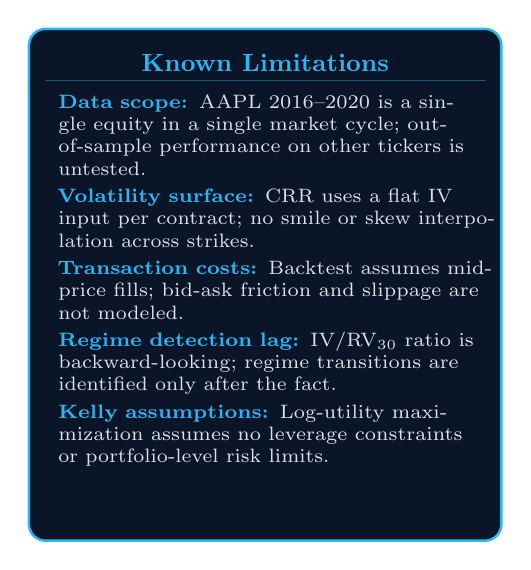
\begin{tikzpicture}
        \fill[navydark,rounded corners=6pt] (0,0) rectangle (6.0,6.5);
        \draw[skyblue,line width=0.9pt,rounded corners=6pt]
          (0,0) rectangle (6.0,6.5);

        \node[text=skyblue,font=\small\bfseries,anchor=north]
          at (3.0,6.3) {Known Limitations};
        \draw[skyblue,opacity=0.4] (0.2,5.85) -- (5.8,5.85);

        \node[text=silvergray,font=\scriptsize,anchor=north west,
              text width=5.5cm,align=left]
          at (0.25,5.78)
          {\textbf{\textcolor{skyblue}{Data scope:}} AAPL 2016--2020 is
           a single equity in a single market cycle; out-of-sample
           performance on other tickers is untested.\\[2pt]
           \textbf{\textcolor{skyblue}{Volatility surface:}} CRR uses
           a flat IV input per contract; no smile or skew
           interpolation across strikes.\\[2pt]
           \textbf{\textcolor{skyblue}{Transaction costs:}} Backtest
           assumes mid-price fills; bid-ask friction and slippage
           are not modeled.\\[2pt]
           \textbf{\textcolor{skyblue}{Regime detection lag:}}
           IV/RV\textsubscript{30} ratio is backward-looking;
           regime transitions are identified only after the fact.\\[2pt]
           \textbf{\textcolor{skyblue}{Kelly assumptions:}}
           Log-utility maximization assumes no leverage constraints
           or portfolio-level risk limits.};
      \end{tikzpicture}
    \end{column}
  \end{columns}
\end{frame}

% ══════════════════════════════════════════════════════════════════════════════
%  SLIDE 7A — LIVE DEMO: INTERACTIVE CRR BINOMIAL PRICING CALCULATOR
% ══════════════════════════════════════════════════════════════════════════════
\begin{frame}{Live Demo --- Interactive CRR Binomial Pricing Calculator}
  \begin{tikzpicture}[remember picture,overlay]
    \gridbackground
  \end{tikzpicture}

  \vspace{-0.4em}
  {\footnotesize\textcolor{authorgray}{Streamlit application\hspace{1em}$\cdot$\hspace{1em}%
   runs locally on any laptop with Python 3.13\hspace{1em}$\cdot$\hspace{1em}%
   ticker-agnostic}}

  \vspace{0.4em}
  \begin{columns}[T]
    \begin{column}{0.58\textwidth}
      \centering
      \adjustbox{max width=\linewidth,max height=5.8cm,keepaspectratio}{%
        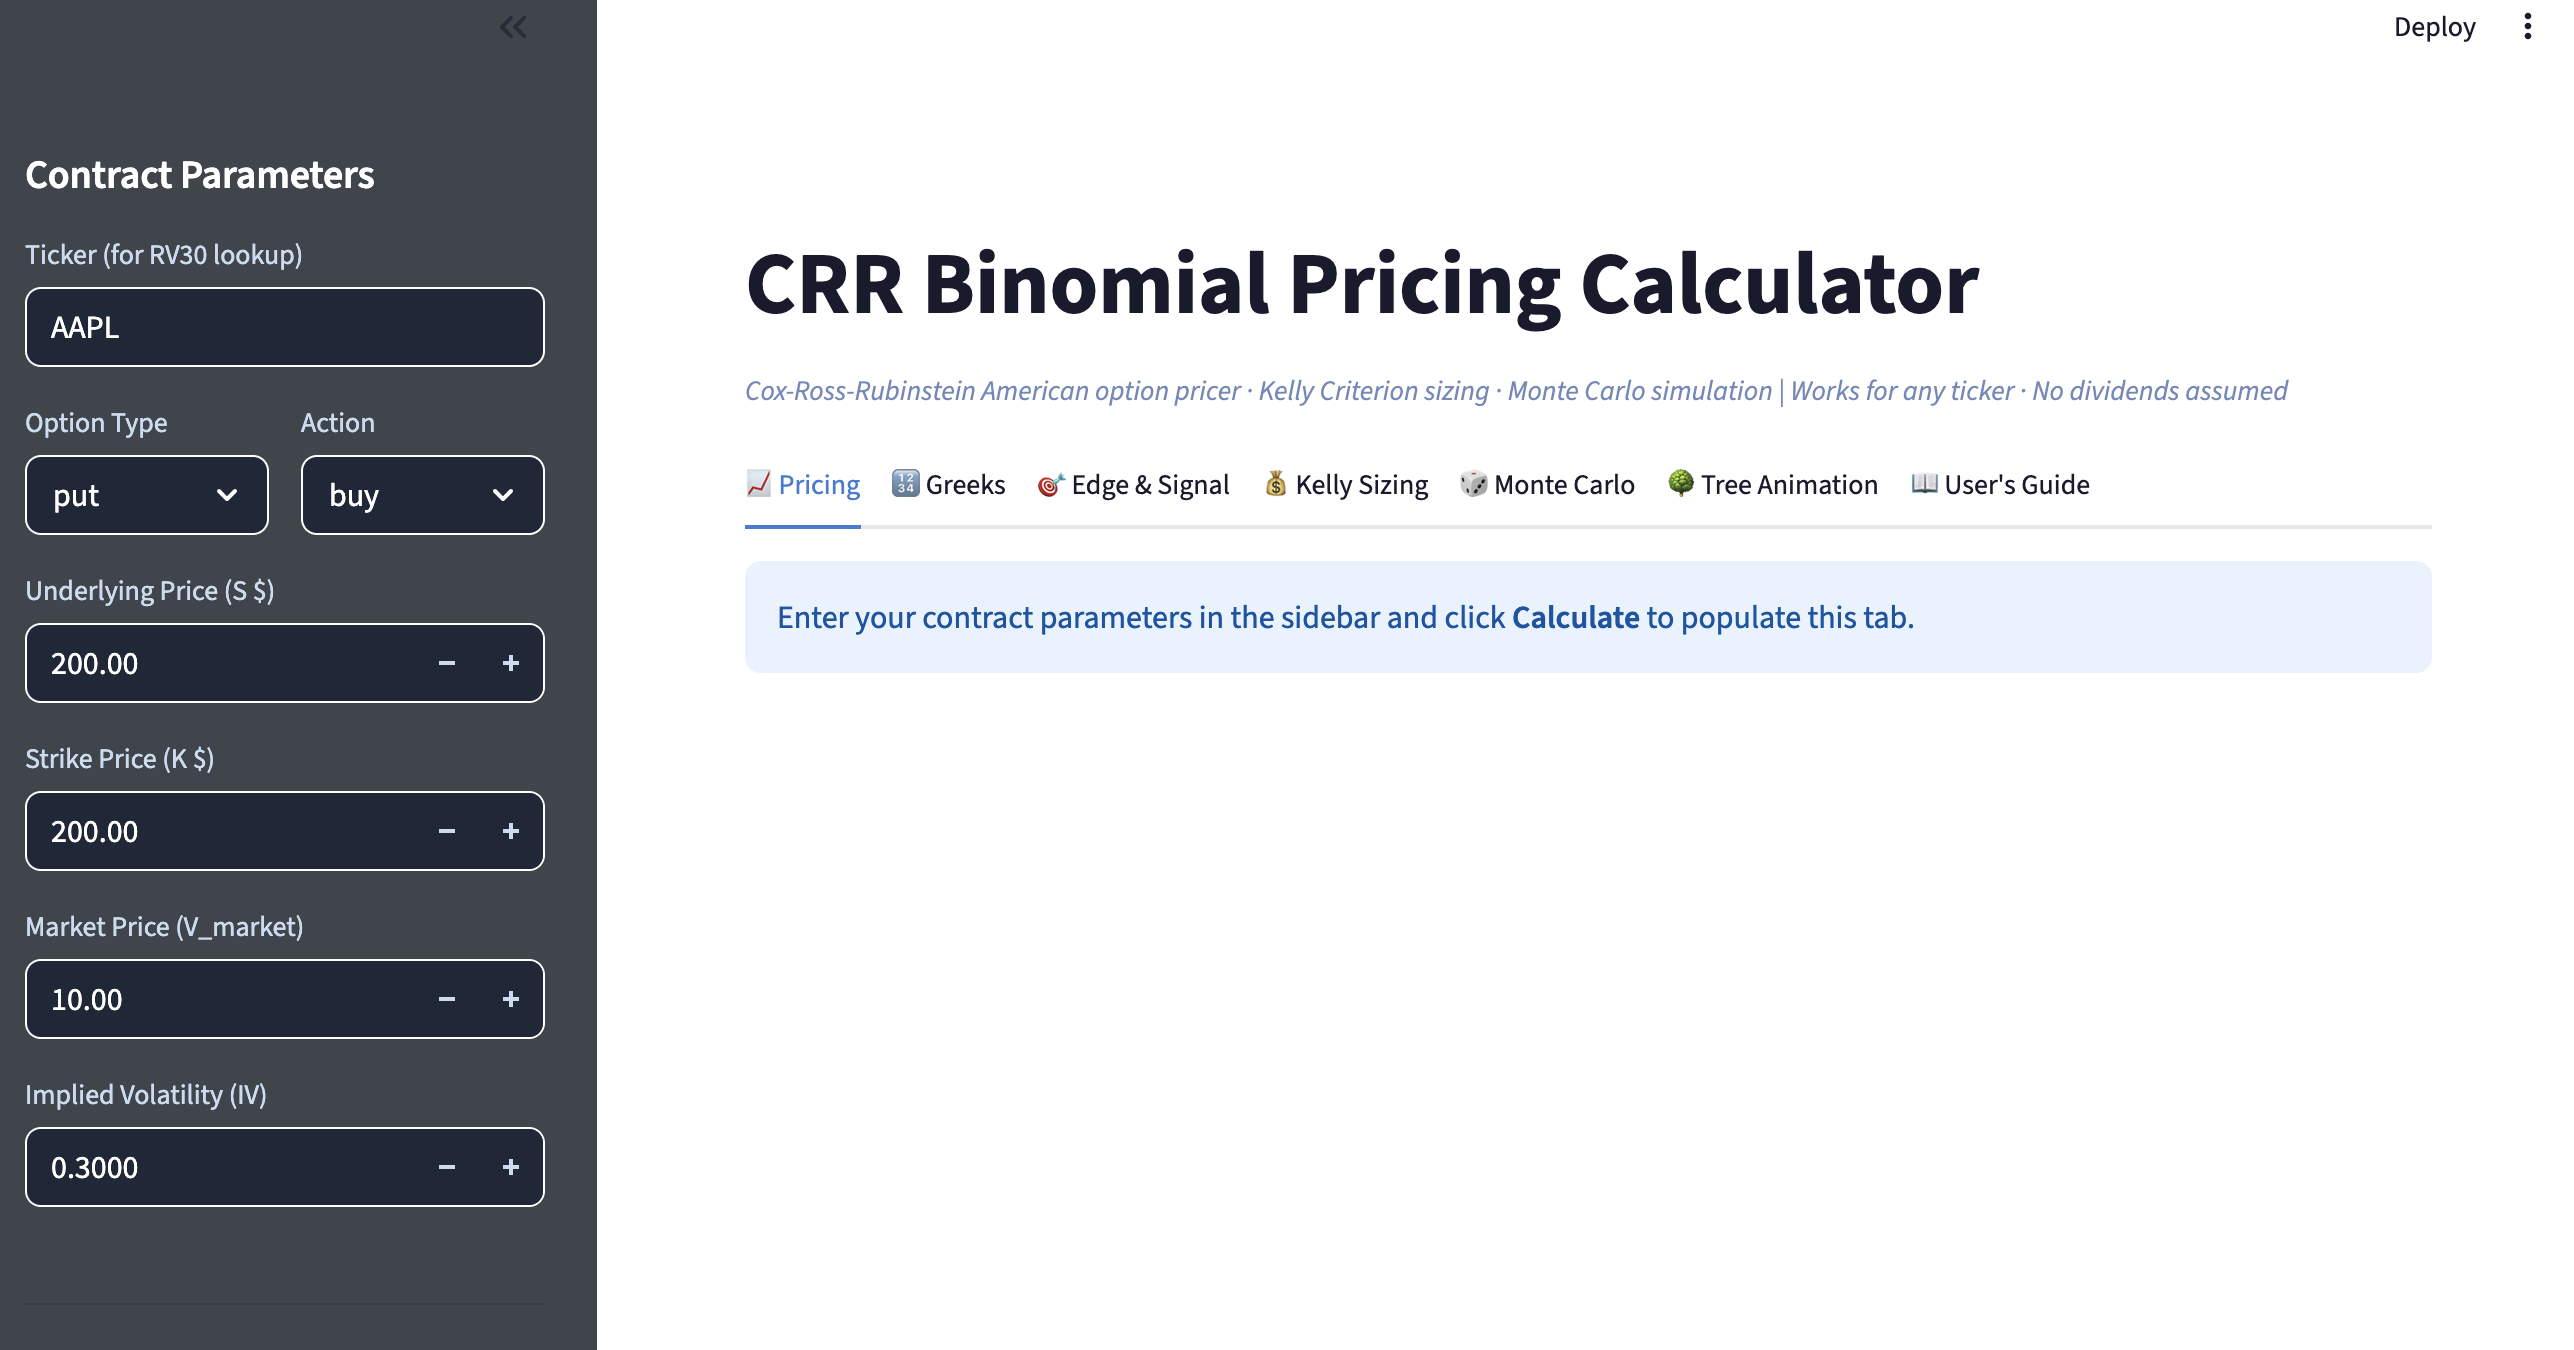
\includegraphics{previews/crr-binomial-pricing-calculator.png}}
    \end{column}

    \begin{column}{0.40\textwidth}
      \vspace{0.4em}
      \textbf{\textcolor{navymid}{Demo plan (next 3 minutes)}}\\[6pt]
      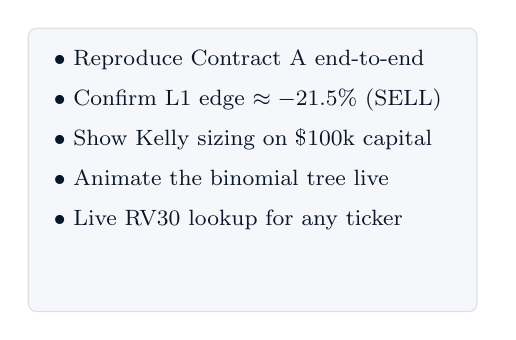
\begin{tikzpicture}
        \fill[whitesmoke,draw=silvergray,rounded corners=3pt]
              (0,0) rectangle (5.7,3.6);
        \node[anchor=north west,text=navydark,font=\footnotesize,
              text width=5.4cm,align=left]
          at (0.2,3.45)
          {$\bullet$~Reproduce Contract A end-to-end\\[5pt]
           $\bullet$~Confirm L1 edge $\approx -21.5\%$ (SELL)\\[5pt]
           $\bullet$~Show Kelly sizing on \$100k capital\\[5pt]
           $\bullet$~Animate the binomial tree live\\[5pt]
           $\bullet$~Live RV30 lookup for any ticker};
      \end{tikzpicture}
    \end{column}
  \end{columns}
\end{frame}

% ══════════════════════════════════════════════════════════════════════════════
%  SLIDE 8 — CONCLUSION
% ══════════════════════════════════════════════════════════════════════════════
\begin{frame}{Conclusion}
  \gridbackground

  % Central contribution statement
  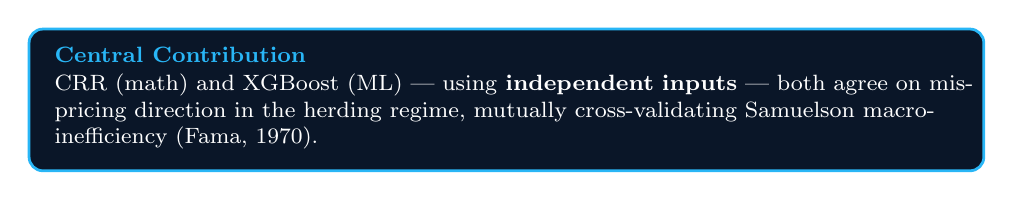
\begin{tikzpicture}
    \fill[navydark,rounded corners=5pt] (0,0) rectangle (\textwidth,1.80cm);
    \draw[skyblue,line width=1pt,rounded corners=5pt]
      (0,0) rectangle (\textwidth,1.80cm);
    \node[text=skyblue,font=\footnotesize\bfseries,anchor=north west]
      at (0.2,1.70) {Central Contribution};
    \node[text=white,font=\footnotesize,anchor=north west,
          text width=\dimexpr\textwidth-0.4cm\relax,align=left]
      at (0.2,1.35)
      {CRR (math) and XGBoost (ML) --- using \textbf{independent inputs}
       --- both agree on mispricing direction in the herding regime,
       mutually cross-validating Samuelson macro-inefficiency (Fama, 1970).};
  \end{tikzpicture}

  \vspace{0.15em}
  \textbf{\textcolor{navymid}{\footnotesize Hypotheses Confirmed}}
  \vspace{0.05em}

  \begin{tikzpicture}[
      hbox/.style={rounded corners=3pt,inner xsep=8pt,inner ysep=4pt,
                   align=left,text width=\dimexpr\textwidth-0.6cm\relax,
                   font=\scriptsize}]

    \node[hbox,fill=navymid,text=white] (h1) at (0,0) {%
      \textcolor{skyblue}{\bfseries H1 — CRR Benchmark Confirmed.}
      Model within 1--2\% of market mid on 80\% of AMD live-chain
      contracts; sub-rounding precision validates CRR as fair-value reference.};

    \node[hbox,fill=forestgreen,text=white,below=0.10cm of h1] (h2) {%
      \textcolor{skyblue}{\bfseries H2 — XGBoost Independent Estimator Confirmed.}
      Brier score 0.211 $<$ 0.25 naive baseline; top features are moneyness
      and Days to Expiration (DTE) — no implicit IV leakage.};

    \node[hbox,fill=burntorange,text=white,below=0.10cm of h2] (h3) {%
      \textcolor{skyblue}{\bfseries H3 — Fractional Kelly Dominates Confirmed.}
      \$2.9M P\&L over 101{,}535 AAPL contracts (2016--2020);
      max drawdown $<$15\%, circuit breaker never triggered.};
  \end{tikzpicture}

  \vspace{0.15em}
  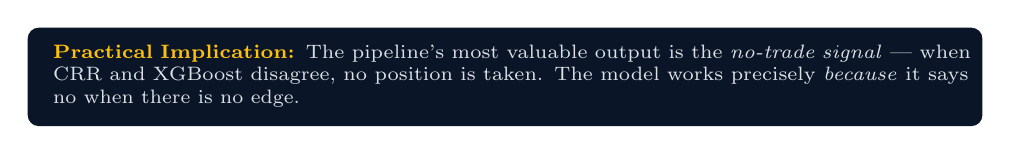
\begin{tikzpicture}
    \fill[navydark,rounded corners=4pt] (0,0) rectangle (\textwidth,1.25cm);
    \node[text=silvergray,font=\scriptsize,anchor=north west,
          text width=\dimexpr\textwidth-0.4cm\relax,align=left]
      at (0.2,1.15)
      {\textbf{\textcolor{goldaccent}{Practical Implication:}} The
       pipeline's most valuable output is the \emph{no-trade signal}
       — when CRR and XGBoost disagree, no position is taken. The
       model works precisely \emph{because} it says no when there
       is no edge.};
  \end{tikzpicture}
\end{frame}

\end{document}
